\documentclass[a4paper,11pt]{report}

\usepackage{courier}
% makes listings look much nicer, and also 
% makes keywords in listings boldface (as they should be)

\usepackage{user-guide} % custom style

\makeatletter
\@ifpackageloaded{tex4ht}{%
	% packages/options only used for generating html
	\usepackage{graphicx}	
	
}{%
	% packages/options only used for generating pdf
	\usepackage[pdftex]{graphicx}

	% NextFile is defined by tex4ht, replace it with a NOOP if not generating html
	\newcommand{\NextFile}[1]{}

}
\makeatother

\usepackage[normalem]{ulem}

%%%%%%%%%%%%%%%%%%%%%%%%%%%%%%%%%%%%%%%%%%%%
%%%%%%%%%%%%%%%%%%%%%%%%%%%%%%%%%%%%%%%%%%%%
\usepackage[dvipsnames,svgnames]{xcolor}

\usepackage{soul}

%%%%%%%%%%%%%%%%%%%%%%%%%%%%%%%%%%%%%%%%%%%%
%%%%%%%%%%%%%%%%%%%%%%%%%%%%%%%%%%%%%%%%%%%%

\usepackage[utf8]{inputenc}

\usepackage{tabularx}

%%%%%%%%%%%%%%%%%%%%%%%%%%%%%%%%%%%%%%%%%%%%
%%%%%%%%%%%%%%%%%%%%%%%%%%%%%%%%%%%%%%%%%%%%
\usepackage{listings}

\lstset{language=java,basicstyle=\ttfamily\footnotesize,lineskip=-1pt,keywordstyle=\bfseries\color{blue},commentstyle=\bfseries\color{red},stringstyle=\bfseries\color{ForestGreen},morekeywords={Link,Node,Vehicle},showstringspaces=false,frame=none}
\lstset{language=XML,basicstyle=\ttfamily\footnotesize,tabsize=3,lineskip=-1pt,keywordstyle=\bfseries\color{blue},commentstyle=\bfseries\color{red},stringstyle=\bfseries\color{ForestGreen},showstringspaces=false,frame=none}
% these are my own colors but I am not militant about them.
% I am also not militant about the morekeywords.
% I am, however, somewhat militant about ttfamily font. 
% kai, jul'13


% looks like a bug that listings cannot be defined to be floating except by defining a new environment
% work-around from http://tex.stackexchange.com/questions/43509/lstlisting-ignores-float-setting
\lstnewenvironment{xml-file}[1][]
  {\lstset{language=XML,float=thb,frame=tb,#1}}% \begin{xml-file}[...]
  {} % \end{javalisting}



%%%%%%%%%%%%%%%%%%%%%%%%%%%%%%%%%%%%%%%%%%%%
%%%%%%%%%%%%%%%%%%%%%%%%%%%%%%%%%%%%%%%%%%%%
%% \usepackage{a4wide}
\usepackage{geometry}
\geometry{a4paper,headsep=4mm,top=15mm,bottom=2cm,left=2.0cm,right=3.0cm}

\parindent0pt
\parskip0.3\baselineskip
%%%%%%%%%%%%%%%%%%%%%%%%%%%%%%%%%%%%%%%%%%%%
%%%%%%%%%%%%%%%%%%%%%%%%%%%%%%%%%%%%%%%%%%%%
\usepackage{fancyhdr}
% needs to be after geometry!
 
\lhead{\let\uppercase=\relax\sf\footnotesize\leftmark}
\chead{}
\rhead{\let\uppercase=\relax\sf\footnotesize\rightmark}

\pagestyle{fancy}

\renewcommand{\chaptermark}[1]{%
%
\markboth{\thechapter.\ #1\\}{}
%
}

\renewcommand{\sectionmark}[1]{%
%
\markright{\thesection.\ #1}
%
}
%%%%%%%%%%%%%%%%%%%%%%%%%%%%%%%%%%%%%%%%%%%%
%%%%%%%%%%%%%%%%%%%%%%%%%%%%%%%%%%%%%%%%%%%%
\newcommand{\myemph}[1]{\textcolor{red}{\emph{#1}}}

\newcommand{\todo}[1]{\hl{\emph{TODO #1}}}

\newcommand{\kai}[1]{\textcolor{blue}{[[#1 kai]]}}

\newcommand{\authorsOfDoc}[1]{\vspace{-.5em}\centerline{\hfill Author(s) of this document: #1}\medskip}
\newcommand{\authorsOfCode}[1]{\vspace{-.5em}\centerline{\hfill Main author(s) of the code: #1}\medskip}
\newcommand{\maintainers}[1]{\vspace{-.5em}\centerline{\hfill Maintainer(s): #1}\medskip}

%%%%%%%%%%%%%%%%%%%%%%%%%%%%%%%%%%%%%%%%%%%%
%%%%%%%%%%%%%%%%%%%%%%%%%%%%%%%%%%%%%%%%%%%%
\usepackage{hyperref}
% hyperref needs to be late in calling sequence!


\def\umbruch{\vfill\eject}
\def\umbruch{\relax}

\def\configOptionsNote#1{%
%
\begin{note}
Look into the file {\tt output\_config.xml.gz} in the section {\tt #1} for configuration options.
\end{note}
%
}

%%%%%%%%%%%%%%%%%%%%%%%%%%%%%%%%%%%%%%%%%%%%
%%%%%%%%%%%%%%%%%%%%%%%%%%%%%%%%%%%%%%%%%%%%
%%%%%%%%%%%%%%%%%%%%%%%%%%%%%%%%%%%%%%%%%%%%
%%%%%%%%%%%%%%%%%%%%%%%%%%%%%%%%%%%%%%%%%%%%

\begin{document}
\NextFile{index.html}
\tolerance10000

\title{MATSim User Guide}

\author{%
Marcel~Rieser, % first
%
% everybody in between alphabetic???
Christoph~Dobler,
Thibaut~Dubernet,
Dominik~Grether,
Andreas~Horni, 
Gregor~Lämmel,
Rashid~Waraich,
Michael~Zilske,
%
Kay~W.~Axhausen, % second-last
Kai~Nagel % last
}

\begin{titlepage}
\makeatletter
%\pdfbookmark[1]{Title}{bookmark:Title}
\pagestyle{empty}

\definecolor{Dark}{gray}{.2} 
\definecolor{Medium}{gray}{.55} 
\definecolor{Light}{gray}{.8} 

\makebox(0,0){} % for some strange reason needed, otherwise vfill has no effect
\vspace{3cm}
\par
\raggedright
{\textcolor{Medium}{\fontsize{45}{60}\sffamily\bfseries \@title}}\par
\vspace{1cm}
% {\textcolor{Medium}{\titleFontSmall Release Fall 2014 (Version 0.6.0)}}\par
{\textcolor{Medium}{\titleFontSmall Development Version\\last updated \@date}}\par
\vspace{15cm}
{\titleFontSmall \mdseries\par\@author}\\
\vspace{2cm}
\raggedleft

\includegraphics[width=.33\textwidth]{figures/MATSimLogo_blue.png}

\makeatother
\end{titlepage}
% \maketitle

\umbruch

\section*{Note}

The material found in this document was originally maintained as a collection of web pages.  Those were eventually automatically converted to latex, and incrementally cleaned up since then.  

As a result, leftovers from those web pages can still be found in the document, including lots of links to web pages which could be replaced by internal links in the document, and links to web pages where the material should be inlined into the document.
\\
\hrule

Originally generated 2013-06-12T12:13:34+02:00
\\from matsim.org/docs/userguide
\\but changed since then.



\umbruch

\tableofcontents


%%%%%%%%%%%%%%%%%%%%%%%%%%%%%%%%%%%%%%%%%%%%
%%%%%%%%%%%%%%%%%%%%%%%%%%%%%%%%%%%%%%%%%%%%
\NextFile{Introduction.html}
\chapter{Introduction}

\authorsOfDoc{Marcel Rieser}
 
\bigskip

\section{What is MATSim?}

MATSim provides a framework to implement large-scale agent-based transport
simulations. The framework consists of severel modules which can be combined or
used stand-alone. Modules can be replaced by own implementations to test single
aspects of your own work. Currently, MATSim offers a framework for
demand-modeling, agent-based mobility simulation (traffic flow simulation),
re-planning, a controller to iteratively run simulations as well as methods to
analyze the output generated by the modules.

The basic set of features of MATSim can be used just by using the software as
is, providing your own input data and just modifying the configuration for the
simulation. For advanced usages, it is necessary to write your own program code
that integrates with MATSim, e.g. to provide special functionality or have your
custom analysis output.


\section{Features}

The following list shows the key features of MATSim:

\begin{description}\styleItemize
\item[Agent-Based, Multi-Modal Simulation of Daily Mobility Behavior.] MATSim is
capable of simulating private car traffic and public transport in large detail, and is able
to support additional modes (e.g. pedestrians or cyclists) as well. Simulations
typically cover one full day, and the mobility behaviour of a large number of
single persons (``agents'') is simulated simultaneously. This allows to track
single agents through their whole day, from \emph{home} to \emph{work}, to
\emph{leisure} or \emph{shopping} and back to \emph{home}.

\item[Fast, even for Large Scenarios.] MATSim is able to simulate scenarios with
several millions agents on networks with hundreds of thousands of road segments.
All you need is a current, fast desktop computer with enough memory. Even in
such cases, MATSim often only takes a couple of minutes for the simulation of
one complete day.

% \item[Sophisticated Interactive Visualizer]  Forget aggregated results!
% MATSim provides a fast Visualizer that can  display the location of each agent
% in the simulation and what it is  currently doing. It can even connect to a
% running simulation, allowing  interactively querying agents' states,
% visualizing agents' routes or  perform live analyses of the network state.

\item[Versatile Analyses and Simulation Output.]
During the simulation, MATSim collects several key values from the 
simulation and outputs them to give you a quick overview of the current state
of the simulation. Among other results, it can compare the simulated traffic to
real world data from counting stations, displaying the results interactively in
Google Earth. Additionally, MATSim provides  detailed output from the traffic
simulation, which can easily be parsed by other applications to create
your own special analyses.

\item[Modular Approach.] MATSim allows for easy replacement or addition of
functionality. This allows you to add your own algorithms for agent-behavior
and plug them into  MATSim, or use your own transport simulation while using
MATSim's replanning features.

\item[Open Source \& Multi-Platform.]
MATSim is  distributed under the Gnu Public License (GPL), which means that
MATSim  can be downloaded and used free of charge. Additionally, you get the 
complete source code which you may modify within certain constraints  (see the
license for more details). Written in Java, MATSim runs on all  major operating
systems, including Linux, Windows and Mac OS X.

\item[Active Development and Versatile Usage of MATSim.]
Researchers from several locations are currently working on MATSim. Core
development takes place world wide, with the efforts lead by the Berlin
Institute of Technology (TU Berlin), the Swiss Federal Institute of Technology
(ETH) in Zurich, as well as Senozon, a private company founded by two former PhD students.
Additional development (as far as we are aware of) currently takes place in
South Africa, Germany, Canada as well as other places around the world. This
distribution of development ensures that MATSim not only works for one
scenario/context, but can be adapted to many different scenarios.
\end{description}

\section{About this Guide}

This user guide should help you to get started with MATSim. 
It starts by giving a broad overview of MATSim, highlighting the different parts
of MATSim and how they work together in Chpt.~\ref{sec:Overview}. In
Chpt.~\ref{sec:Terminology}, Terminology, some terms commonly referred to in
this user guide are explained and put into relation to terms used to
describe similar concepts. After this, you're ready to start MATSim for the
first time! Chpt.~\ref{sec:Running} shows you how to do this in a number of
different environments. If you're interested to build your own scenario, you'll
find Chpt.~\ref{sec:BuildingScenarios} helpful. It explains what data and in
what format is necessary to build a scenario.

\todo{MR}
\NextFile{Overview.html}
\chapter{Overview}
\label{sec:Overview}

\authorsOfDoc{Marcel Rieser}
 
\bigskip

\begin{chapter-intro}
This chapter gives an overview of the major components of MATSim and how they
work together, essentially building the foundation for the MATSim framework.
\end{chapter-intro}

\section{The Major Stages of a MATSim Simulation}

In a typical MATSim simulation, travel demand data is simulated and optimized on
a given transportation network (e.g. a road network, or a multimodal network in
the case when public transport is also considered in the simulation).
The optimization of the demand data is one of the key features of MATSim, making
it suitable to be used for policy studies. In this whole simulation and
optimization process, 5 major stages can be identified:
\begin{itemize}\styleItemize
	\item initial demand
	\item execution
	\item scoring
	\item replanning
	\item analysis
\end{itemize}

These 5 stages are executed in the order shown in
Fig.~\ref{fig:overview:controllerFlow}.
In the following, the responsibilities of each stage is shortly described. The
details for the stages, including what options are available to influence the
stages and how they work, are explained in separate chapters later on.


\begin{figure}[htp]
\begin{center}
  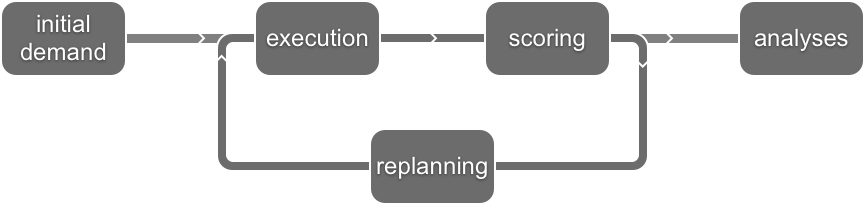
\includegraphics[width=.8\textwidth]{figures/overview/controllerFlow.png}
  \caption{Stages of a MATSim Simulation}
  \label{fig:overview:controllerFlow}
\end{center}
\end{figure}

\paragraph{Initial demand:}
The initial demand describes the mobility behaviour to be simulated. It contains
the full list of agents, and for each agent at least one day plan. A day plan
contains a list of activities (e.g. being \emph{home}, being at \emph{work}) and
trips (e.g. going \emph{by car} to shopping) along with temporal information
(e.g. leaving home \emph{at 7:23 am}, working \emph{until 5:39 pm}) and
additional information (e.g. detailed route going from home to work). Plans
describe the intentions of agents. If agents calculate too optimistically, get
stuck in a traffic jam or miss a bus, it might be that their plan cannot be
realized in the simulation as the agents intended to.

\paragraph{Execution:}
Often also called the \emph{mobility simulation} (or just \emph{mobsim}), the
agents' plans get executed along each other in a representation of the physical
world. This means that the agents and their vehicles are moved around in the
network (the \emph{infrastructure} in the real world). During this execution of
the plans, agents can influence each other by taking up space in the virtual
world. If too many agents want to travel on the same road at a specific time,
they generate a traffic jam in the mobility simulation. This is why the agents'
plans only describe their intentions for a day, but do not actually describe
their day.

\paragraph{Scoring:}
Once the execution of the plans finished, the agents' plans are evaluated based
on their experienced execution. The exact scoring function is customizable, but
generally time spent at activities increases the score, while time spent
travelling decreases it. Agents stuck in a traffic jam thus loose points, while
agents with short and quick trips are able to accumulate more score points by
performing activities for a longer time period.

\paragraph{Replanning:}
As mentioned in the execution stage, agents can be influenced by others and, for
example, get stuck in a traffic jam. During the replanning stage, agents may
modify their plans (actually, they modify copies of the plans, see
Sec.~\ref{sec:Overview:Optimization}) in order to try to avoid situations in the
mobility simulation that lead to bad scores. Typical examples of such
modifications are the modification of activity end times, effectively changing
the start time of the following trip, changing the mode of transport for a trip,
or changing the route for a trip (departure time choice, mode choice, route
choice). In MATSim, these modifications are performed by so-called
\emph{Strategy Modules}.

\paragraph{Analysis:}
At the end of a complete simulation, one is often interested in some key
performance values of the simulation. Examples could be mode shares, miles
travelled in total by all agents, or average trip duration and distance per
mode and hour. Such analyses could either be automatically be performed at then
end, or in a separate post-processing step.

\bigskip

The three stages Execution, Scoring and Replanning are performed iteratively in
order to give the agents multiple opportunities to adapt their plans to the
plans and behaviour of the other agents. This is why MATSim typically performs
multiple \emph{iterations} within one simulation run, consisting of multiple
mobility simulation, scoring and replanning executions, until the end result is
available.

MATSim provides a \emph{Controller} (sadly misspelled as \emph{Controler} in
some places) which implements the iteration loop as shown in
Fig.~\ref{fig:overview:controllerFlow}. This Controller is typically the entry
point for running MATSim simulations, as it handles all aspects from loading all
the required data, configuring the whole setup according to the user's settings,
and iteratively calling the execution, scoring and re-planning stages.
Chpt.~\ref{sec:Running} shows the usage of the Controller in more
detail.


\section{The Optimization Process}
\label{sec:Overview:Optimization}

As outlined above, agents can modify the plans from the initial demand to try to
come up with new variants of the plan that lead to higher scores. The main
concept of the optimization process follows the principles of so-called
\emph{(co-)evolutionary algorithms}. Evolutionary algorithms typically maintain
a set of candidates which are evaluated using a fitness function. New candidates are
generated and evaluated. If they have a bad fitness, they are discarded. If they
have a good fitness, another candidate with a worse fitness is removed from the
set of candidates and the new candidate is added to the set. This is repeated
until no new good candidates are found after some tries.

MATSim implements an evolutionary algorithm for each agent. As all agents are
optimized using their own evolutionary algorithm, the whole system is called a
co-evolutionary algorithm. The set of candidates corresponds to the set of plans
each agent has. New candidates are generated in the replanning stage by making a
copy of an existing plan and modifying the copy. The fitness evaluation is done
by scoring the execution of the plan.
Thus, the replanning stage in MATSim corresponds to the generation of new
candidates of evolutionary algorithms, while the execution and scoring of plans
corresponds to the evaluation of the fitness of the candidates. The repetition 

With each iteration, the goal is that the average score of the executed plans
increase, corresponding to the agents improving their plans such that they can
perform their daily activities as good as possible.
Fig.~\ref{fig:overview:scores} shows how the average score develops in a typical
MATSim simulation over the course of the iterations. Note that the absolute
value of the scores may depend upon the scenario. As can be nicely seen in the
figure, the average executed score typically improves very rapidly in the first
few iterations, but will only improve very slightly in later iterations or even
degrade a few times.


\begin{figure}[htp]
\begin{center}
  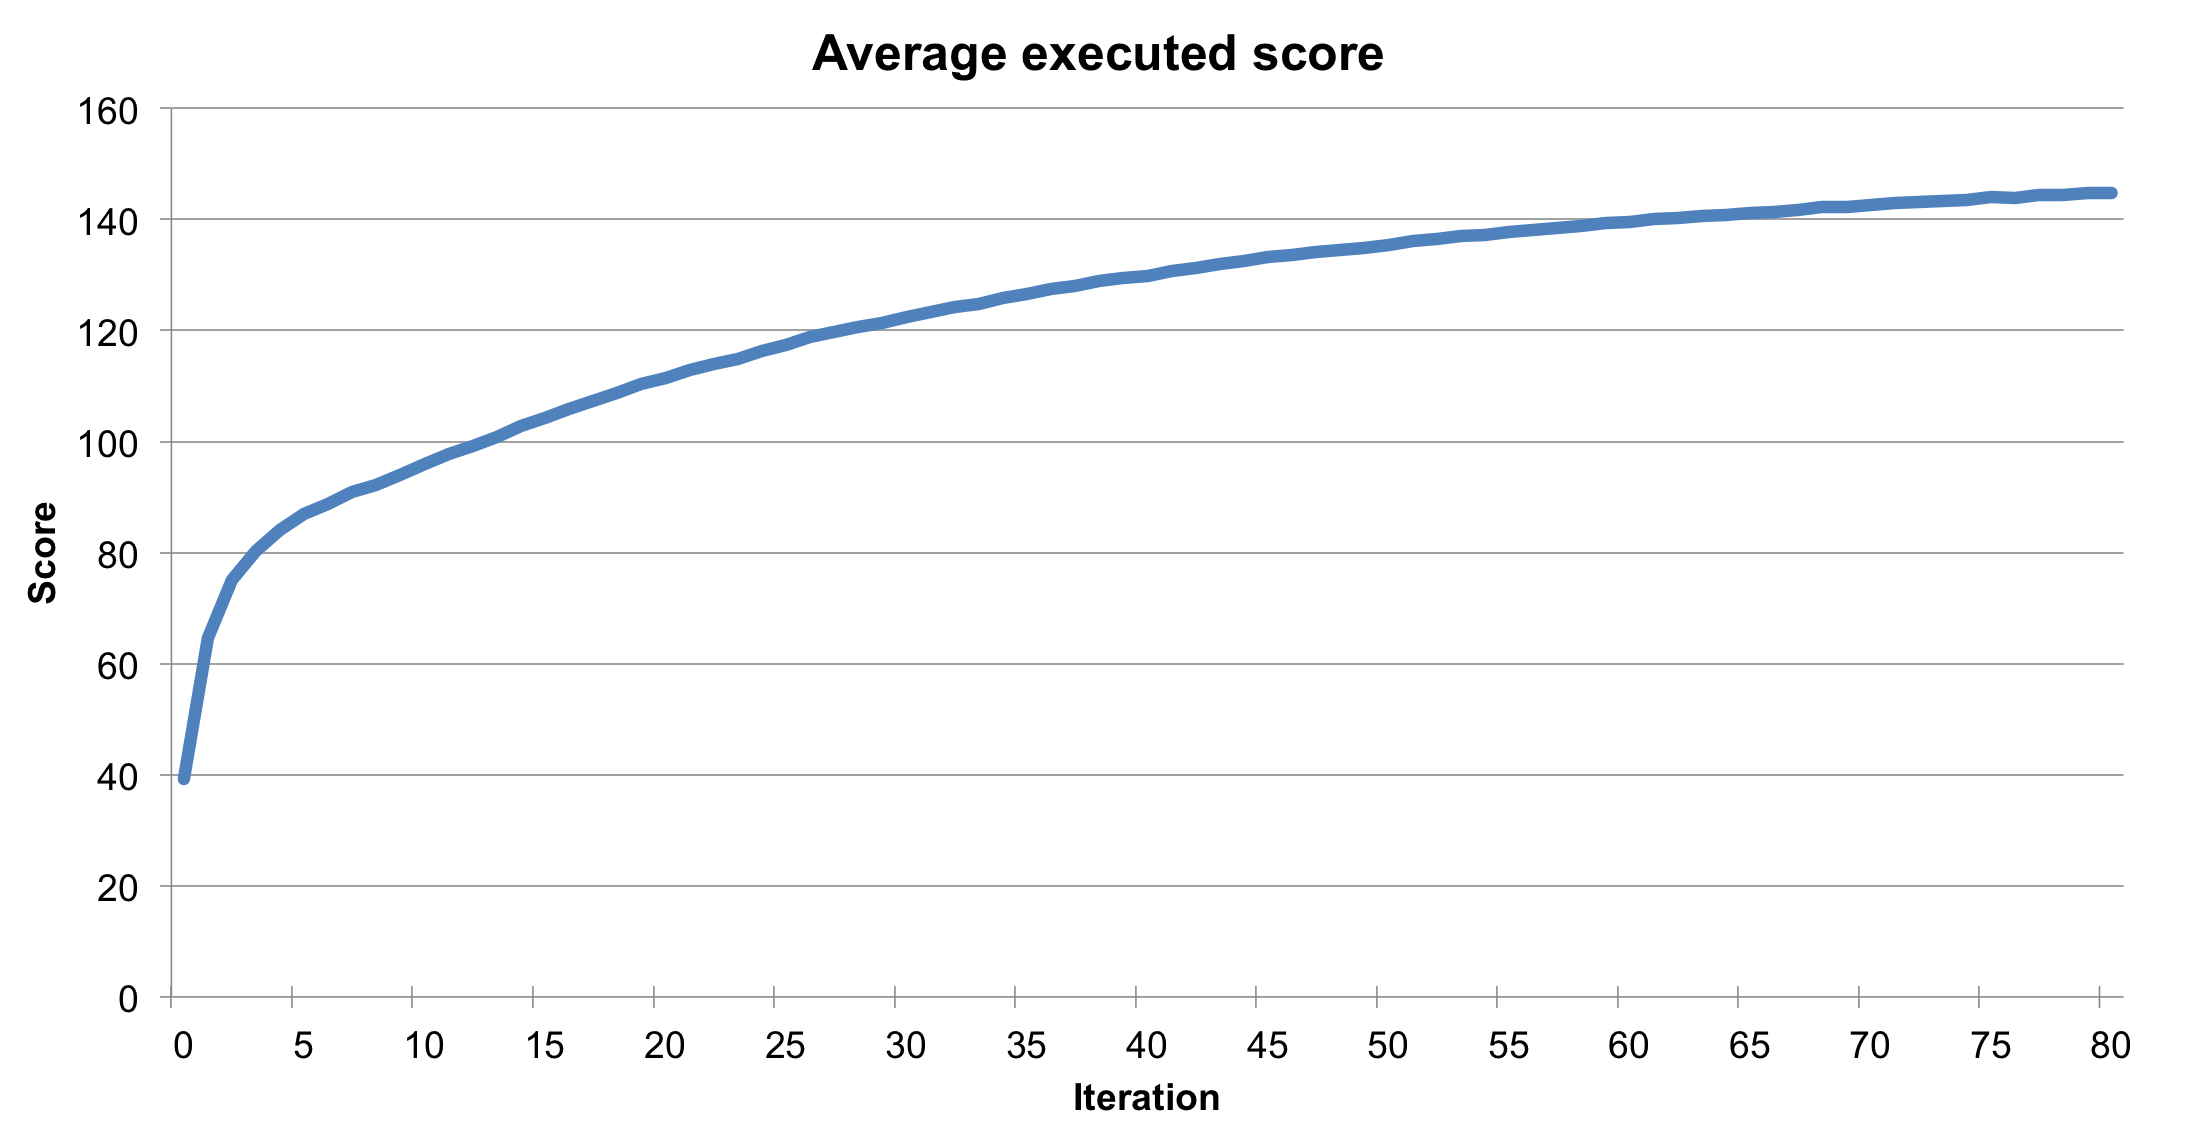
\includegraphics[width=.9\textwidth]{figures/overview/scorestats.png}
  \caption{Tpyical development of the average score of the executed plans over
  the iterations}
  \label{fig:overview:scores}
\end{center}
\end{figure}


\section{Mobility Simulation Events}
The mobility simulation moves the agents around in the virtual world according
to their plans and within the bounds of the ``simulated reality''. The
mobility simulation documents its moves with so-called ``Events''. These events
are small pieces of information describing the action of an object at a
specific time. Examples of such events can be:
\begin{itemize}\styleItemize
  \item An agent finishes an activity
  \item An agent starts a trip
  \item A vehicle enters a road segment
  \item A vehicle leaves a road segment
  \item An agent bordes a public transport vehicle
  \item An agent arrives at a location
  \item An agent starts an activity
\end{itemize}
Each event has a timestamp, a type, and additional attributes required to
describe the action like the agent's id, a link id, an activity type or other
data. In theory, it should be possible to replay the mobility simulation just by
the information stored in the events. While plans describe the agents' plan for
a day, the events describe how the agents' day actually was (according to the
simulation).

As the events are so basic, each agent typically generates hundreds of events
during one execution of a mobility simulation. In total, the number of events
generated by a mobility simulation can easily reach a million or more, with
large simulations even generating more than a billion events. But as the events
really describe all the details from the execution of the plans, it is possible
to extract mostly any kind of aggregated data one is interested in. Practically
all analyses of MATSim simulations make use of events to calculate some data.
Examples of such analyses are the average duration of an activity, average trip
duration or distance, mode shares per time window, number of passengers in
specific transit lines and many more.

The scoring of the executed plans makes use of events to find out how much time
agents spent at activities or for travelling. Some replanning modules might
make use of events as well: The router for example can use the information
contained in events to figure out what links are jammed at certain times and
route agents around that jam when creating new plans.


\section{Customizability}
MATSim is designed to be modular. Nearly all parts can be customized, replaced
or enhanced with custom functionality. Some customizations are easier than
others. Replacing the mobility simulation for additional behaviour might be one
of the hardest things to achieve, because a lot of functionality would have to be re-implemented. Changing the replanning on the other hand is
quite easy, especially as there is already a number of modules available for
different replanning needs which can be activiated and used without programming
and only by modifying the configuration file. This guide will mostly focus on
functionality available in a standard release of MATSim that can be used just by
making changes to the configuration file, and not on enhancing MATSim by
programming custom functionality.


\begin{note}
In order to work with MATSim, you should know the \emph{5 major stages} of a
MATSim simulation, why MATSim uses \emph{iterations} and understand conceptually what
data is contained in \emph{plans} and what data is contained in \emph{events}.
\end{note}

\NextFile{Terminology.html}
\chapter{Terminology}
\label{sec:Terminology}

\authorsOfDoc{Kai Nagel}

\bigskip

In  many cases, MATSim uses a terminology that is different from the  mainstream terminology. In most cases, the reason is that the  concepts are only similar, but not identical, and we wanted to avoid the  confusion of using the same term for aspects that are similar but not  identical. The following attempts some commented approximate  "translations" from more standard teminology to MATSim terminology.

\section{Choice set $\to$ ``plan set'' of an agent}

During MATSim iterations, agent accumulate   plans. This can be  interpreted as building a choice set over  time. A  problem is that the  process that generates the choice  set at this  point is not systematic.

\paragraph{Possible future developments:} Once it has been made explicit that "plans generation" means "choice set generation", the terminology may be made standard.

\section{Choice set generation $\to$ Time mutation/re-route/... ; "innovation"}

As said above, the set of MATSim plans can   be seen as this agent's choice set. MATSim generates new plans   "on-the-fly", i.e. while the simulation is running. We sometimes  call  this "innovation", since agents create new plans (= add entries to  the  choice set), rather than choosing between existing plans.

\section{Choice set generation, choice $\to$ replanning}

In MATSim, there is no strict separation between "choice set  generation" and "choice": at the replanning step, for each agent, a  replanning strategy is randomly choosen. This strategy may consist in  selecting a random plan to use to generate a new plan by mutation  ("choice set generation" part), or just to select a past plan based on  the experienced score ("choice" part).

\section{Convergence $\to$ learning rate}

Scores in matsim are computed as
\[
score_{new} = (1-\alpha) \cdot score_{old} +   \alpha \cdot score_{sim} \ , 
\]
where $score_{sim}$ is the score that is obtained from   the execution of the plans (= network loading).

\section{Mu (logit model scaling factor) $\to$ beta\_brain}


MATSim scoring function: 
\[
{\tt BrainExpBeta} \cdot \sum_i \beta_i \, x_i
\]

Typical logit model formulation: 
\[
\mu \cdot \sum_i \beta_i \, x_i
\]

As is well known, $\mu$ or $\beta_i$ are not independently
identifiable from estimation. For simulation, they are hence somewhat
arbitrary. The default value for "BrainExpBeta" is 2 for historical
reasons, but it should be set to 1 if the parameters of the scoring
function are estimated rather than hand-calibrated.

\paragraph{Possible future development:}

Default value of \verb$BrainExpBeta$ should be set to $1.$ instead of $2.$.


\section{Multinomial logit $\to$ ExpBetaPlanSelector}


\paragraph{Comments:}
\begin{itemize}
	\item The main problem is that one needs to keep in mind how the choice set is constructed (see above).
	\item In most simulations, we use ExpBetaPlanChanger instead, which is a   Metropolis Monte Carlo variant of making multinomial logit draws
\end{itemize}

\paragraph{Possible future developments:} None of this is  ideal,  since, after the introduction of a policy, it is not clear which   behavioral switches are due to the policy, and which are due to   sampling. In theory, one should have unbiased samples before and  after  the introduction of the policy, but at this point this is not   implemented and it is also computationally considerably more expensive   than what is done now.

\section{Network loading $\to$ mobsim, mobility simulation, physical simulation}


The standard terminology has the "network   loading" on the "supply  side". In my (KN's) view, the  "simulation of  the physical system" is  not the supply side, but what  in economics is  called "technology". This  can for example be  seen in the fact that  "lane changing" is part of the  mobsim, but this  is, in my view, not a  "supply side" aspect.

\paragraph{Possible future developments:} May switch to "network loading" if there is agreement that this is a better name.

\section{Stationary $\to$ relaxed}

``stationary'' means that the probability   distribution does not shift any  more. However, as long as  "innovation"  is still switched in on MATSim  (new routes, new times,  ...), the  result is not truly stationary. Thus  we avoid the  word. If innovation  is switched off, the result is indeed a   statinary process, but limited  to the set of plans that every agent has   at that point in time.

\paragraph{Possible future developments:} not clear. Minimally, publications should be precise.

\paragraph{Configuration:}
\begin{lstlisting}{language=XML}
<module name="strategy" >
	<!-- iteration after which module will be disabled.  ... -->
	<param name="ModuleDisableAfterIteration_1" value="null" />
	<param name="ModuleDisableAfterIteration_2" value="950" />

	<!-- probability that a strategy is applied to a given person.  ... -->
	<param name="ModuleProbability_1" value="0.9" />
	<param name="ModuleProbability_2" value="0.1" />

	<!-- name of strategy ... -->
	<param name="Module_1" value="ChangeExpBeta" />
	<param name="Module_2" value="ReRoute" />

	<!-- maximum number of plans per agent ... -->
	<param name="maxAgentPlanMemorySize" value="4" />
</module>
\end{lstlisting}


The above means:
\begin{itemize}
	\item StrategyModule "ReRoute" (= innovative Module, produces plans with new routes) is switched off after iteration 950.
	\item StrategyModule "ChangeExpBeta" (= non-innovative Module, switches between existing plans) is never switched off.
	\item If an agent ever ends up with more than 4 plans, plans are deleted  until she is back to 4 plans. (Deletion goes via a  "PlanSelectorForRemoval", which affects the choice set, and thus more  thought needs to go into this. Currently, the plan with the worst  score is removed.)
\end{itemize}

\section{Utility $\leftrightarrow$ score}


At least when using random utility models (such as multinomial logit   aka ExpBeta...), the score has the same function as the deterministic   utility.

\NextFile{RunningMATSim.html}
\chapter{Running MATSim}
\label{sec:Running}

\authorsOfDoc{Marcel Rieser}
 
\bigskip

\begin{chapter-intro}
MATSim comes without any easy to use graphical interface. Instead, it uses text
files for configuration and uses a command line interface to start simulations.
This chapter shows you how to start MATSim simulations in a number of different
computing environments.
\end{chapter-intro}


\section{Prerequisites}

MATSim is written in Java, a programming language which allows to write
applications that run on a large variety of computers. As scenarios can become
quite large, they may consume large amounts of memory (RAM). Very large
scenarios should be run on dedicated servers with enough resources.

In general, to use MATSim, the following requirements must be met:
\begin{itemize}\styleItemize
  \item Java SE 7 must be installed. The latest version of the Java Runtime
  Environment (JRE) can be downloaded from \url{http://java.oracle.com}.
  \item Have at least 2 GB memory for running the examples. For larger
  scenarios, more memory will be required.
  \item Have enough free hard drive space. The provided examples will occupy
  only a few megabytes, but large scenarios can easily use multiple gigabytes of
  disk space.
  \item Last but not least, you need a version of MATSim.
\end{itemize}
This chapter assumes you are using a release (or nightly build) of MATSim which
comes pre-packaged as a jar-file. This chapter will not explain how to compile
and run MATSim based on its program source files. In the remainder of this
chapter, {\tt matsim.jar} will be used to refer to the jar-file of MATSim. The
actual name might differ, e.g. it might include a version number like {\tt
matsim-0.6.0.jar} or {\tt matsim-20140114.jar}.


\section{Using MATSim from a Command Line}
To run MATSim, one needs a configuration file and an estimation, how much memory
the simulation will consume (Don't fear this, you'll get used to this quite
fast). As MATSim comes without graphical user interface, it needs to be run on
the command line. In Linux or Mac OS X, this is typically done using a Terminal
application. In Windows, the Power Shell or Command Prompt can be used.

On the command line, type the following command, but substitute the correct
paths:
\begin{verbatim}
java -Xmx512m -cp /path/to/matsim.jar
      org.matsim.run.Controler /path/to/config.xml
\end{verbatim}
Note that the commands should always be written on one line, they are shown in
this tutorial on multiple lines only for readability.

As an example, on Linux this could look like:
\begin{verbatim}
java -Xmx512m -cp /home/username/matsim/matsim.jar 
      org.matsim.run.Controler /home/user/matsim/input/config.xml
\end{verbatim}

On Mac OS X, it could look like this:
\begin{verbatim}
java -Xmx512m -cp /Users/username/matsim/matsim.jar 
      org.matsim.run.Controler /Users/user/matsim/input/config.xml
\end{verbatim}

On Windows, an example command could be:
\begin{verbatim}
java -Xmx512m -cp C:\MATSim\matsim.jar 
      org.matsim.run.Controler C:\MATSim\input\config.xml
\end{verbatim}

Such a command exists of multiple parts:
\begin{itemize}
  \item {\tt java} tells the system that you want to run Java.
  \item {\tt -Xmx512m} tells Java that it should use up to 512 MB of memory.
  This is typically enough to run the small examples. For larger scenarios, you
  might need more memory: {\tt -Xmx3g} would allow Java to use up to 3 GB of
  memory.
  \item {\tt -cp /path/to/matsim.jar} tells Java where to find the MATSim code.
  \item {\tt org.matsim.run.Controler} tells Java which class (think of ``entry
  point'') it should start running. In most cases, the default MATSim Controler
  is the class you'll need to run simulations.
  \item {\tt /path/to/config.xml} tells MATSim which config file is to be used.
\end{itemize}

In the case you have relative paths in your config file, make sure to start
MATSim in the correct directory. It will interpret all relative paths based on
the directory where the Java process got started, and not where the config file
is located.


\NextFile{BuildingScenarios.html}
\chapter{Building New Scenarios}
\label{sec:BuildingScenarios}

\authorsOfDoc{Marcel Rieser}
 
\bigskip

\begin{chapter-intro}
Starting a new scenario (our term for the application of MATSim to a 
region/area) can appear quite cumbersome at the first glace, as a lot of data
preparation may be required. This chapter gives first an overview of the input
data typically required for running a MATSim scenario, and then gives examples
how such data is generated for existing scenarios.
\end{chapter-intro}


\section{A Minimum Example}

In order to work, MATSim requires at least a network and a travel demand.
Alone with these two inputs and a configuration, MATSim can already be run.

The following section will describe these input data, along with other additional
and optional input data.

\todo{MR Expand this section} 



\section{Typical Input Data Sets}
MATSim uses multiple files to store the different types of data it uses for the
simulation. Tab.~\ref{tab:BuildingScenarios:InputDataSets} gives an
overview over files you may typically encounter when working with MATSim.

Not all files are always required. Very simple simulations can be run
only with a configuration file and the description of the network and
the population containing the agents' plans. For additional functionality, e.g.
for the simulation of public transport, additional files might be required.

\begin{table}[htp]
\begin{tabular}{ll}
\hline
{\tt config.xml}          & configuration options for MATSim \\
{\tt network.xml}         & description of the (road) network \\
{\tt population.xml}      & the travel demand, i.e. the list of agents
and their day plans
\\
{\tt facilities.xml}      & information about locations where
activities can be performed\\
{\tt transitSchedule.xml} & information about transit stop locations
and transit services\\
{\tt transitVehicles.xml} & description of the vehicles used for
public transport services\\
{\tt counts.xml}          & hourly volumes from real-world counting
stations for comparison\\
\hline
\end{tabular}
\caption{Files often used with MATSim}
\label{tab:BuildingScenarios:InputDataSets}
\end{table}

In the following, small examples of these files will be shown and the data they
contain discussed.

\begin{note}
Some of the files, especially {\tt population.xml}, but also {\tt network.xml} 
or {\tt facilities.xml}, might get quite large. To save space, MATSim supports
reading and writing the data in a compressed format. MATSim uses  
GZIP-compression for this. Thus, in many cases, the file names have the 
additional suffix {\tt .gz}, as in {\tt population.xml.gz}. MATSim automatically
detects if files are compressed or should be written compressed based on the 
filename.
\end{note}

\subsection{Configuration}

\begin{xml-file}[caption=An example of a config.xml,
label=lst:BuildingScenarios:configXml]
<?xml version="1.0" ?>
<!DOCTYPE config SYSTEM "http://www.matsim.org/files/dtd/config_v1.dtd">
<config>

	<module name="network">
		<param name="inputNetworkFile" value="example/network.xml" />
	</module>

	<module name="plans">
		<param name="inputPlansFile" value="example/population.xml.gz" />
	</module>

	<module name="controler">
		<param name="outputDirectory" value="./output/" />
		<param name="firstIteration" value="0" />
		<param name="lastIteration" value="10" />
	</module>
	
</config>
\end{xml-file}

The configuration file, often just referred to as \emph{config file}
or as \emph{config.xml}, builds the connection between the user and MATSim.
It contains a list of settings which influence how the simulation behaves.

All configuration parameters are simple pairs of a parameter name and a
parameter value. The parameters are grouped into logical groups. For example,
there is a group with settings related to the Controler like the number of
iterations, or there is another group with settings related to the simulation,
e.g. the end time of the simulation.
Listing~\ref{lst:BuildingScenarios:configXml} shows a very short example of a
configuration file which specifies the network and travel demand data to be used
along with some settings for the Controler.

The list of available parameters and valid parameter values may vary from
release to release. Although we try to keep this stable, due to changes in the
software, most notably by new features, settings may change. To get a list of
all available settings currently available, run the following command:
\begin{lstlisting}
java -cp matsim.jar org.matsim.run.CreateFullConfig fullConfig.xml
\end{lstlisting}
This command will create a new config file {\tt fullConfig.xml} which contains
the full list of available parameters along with their default values. This
makes it easy to see what settings are available. To use and modify certain
settings, the lines with the corresponding parameters can be copied to the
config file specific for the scenario to be simulated and the parameter values
be modified in that file.


\subsection{Network}

\begin{xml-file}[caption=An example of a network.xml,
label=lst:BuildingScenarios:networkXml]
<?xml version="1.0" encoding="utf-8"?>
<!DOCTYPE network SYSTEM "http://www.matsim.org/files/dtd/network_v1.dtd">

<network name="example network">
	<nodes>
		<node id="1" x="0.0" y="0.0"/>
		<node id="2" x="1000.0" y="0.0"/>
		<node id="3" x="1000.0" y="1000.0"/>
	</nodes>
	<links>
		<link id="1" from="1" to="2" length="3000.00" capacity="3600" 
		                           freespeed="27.78" permlanes="2" modes="car" />
		<link id="2" from="2" to="3" length="4000.00" capacity="1800" 
		                           freespeed="27.78" permlanes="1" modes="car" />
		<link id="3" from="3" to="2" length="4000.00" capacity="1800" 
		                           freespeed="27.78" permlanes="1" modes="car" />
		<link id="4" from="3" to="1" length="6000.00" capacity="3600" 
		                           freespeed="27.78" permlanes="2" modes="car" />
	</links>
</network>
\end{xml-file}

The network describes the infrastucture on which the agents (or the vehicles,
respectively), can move around. The network consists of \emph{nodes} and
\emph{links} (in graph theory, these are typically called \emph{vertices} and
\emph{edges}). Listing~\ref{lst:BuildingScenarios:networkXml} shows an example
of a simple description of a network in MATSim's XML data format.

Each element has an identifier \emph{id}. Nodes are described by an X and a Y
coordinate value. Links have more attributes: The \emph{from} and \emph{to}
attribute reference nodes and describe the geometry of the network. Additional
attributes describe the traffic-related aspects of the network:
\begin{itemize}\styleItemize
  \item the \emph{length} of the link, typically in meters (see
  Sec.~\ref{sec:BuildingScenarios:Units}).
  \item the \emph{flow capacity} of the link, i.e. the number of vehicles that
  can pass the link, typically in vehicles per hour.
  \item the \emph{freespeed} is the maximum speed at which vehicles are allowed
  to travel along the link, typically in meters per seconds.
  \item the \emph{number of lanes} ({\tt} permlanes) available in the direction
  specified by the {\tt from} and {\tt to} nodes.
  \item the list of \emph{modes} allowed on the link. This is a comma-separated
  list, e.g. {\tt modes="car,bike,taxi"}.
\end{itemize}
Note that all links are uni-directional. If a road can be travelled in both
directions, two links have to be defined with alternating {\tt to} and {\tt
from} attributes (see links with id {\tt 2} and {\tt 3} in the example given in
Listing~\ref{lst:BuildingScenarios:networkXml}).
Thus, the network can be seen as a directed graph.

\configOptionsNote{network}

\subsection{Demand}

The travel demand for MATSim is described by the agents' day plans. The full set
of agents is typically the \emph{population}, hence the filename {\tt
population.xml}. Alternatively, {\tt plans.xml} is also commonly used in MATSim,
as the population file essentially contains a list of day plans.

The population contains the data in a hierarchical structure, as shown in
Listing~\ref{lst:BuildingScenarios:populationXml}:
\begin{itemize}\styleItemize
  \item The population contains a list of persons.
  \item Each person contains a list of plans.
  \item Each plan contains a list of \emph{Activities} and \emph{Legs}.
\end{itemize}
Exactly one plan per person is marked as \emph{selected}. The selected plan of
each agent is the plan that gets executed by the mobility simulation. During the
replanning stage, a different plan might get marked as being selected. A plan
can contain a score as attribute. The score gets calculated and stored in the
plan during the scoring stage, after the plan was executed by the mobility
simulation.

The list of activities and legs in each plan describe the planned actions by
each agent. Activities have a type assigned and have---except for the last
activity in a day plan---an end time defined (There are some exceptions where
activities have a duration instead of an end time. Such activities are often
automatically generated by routing algorithms and are thus not described in
this guide). To describe the location where an activity takes place, the
activity is either assigned a coordinate by giving an x and y attribute value,
or has a link assigned which describes from which link the activity can be
reached. As the simulation requires the link attribute, the Controler calculates
the nearest link for a given coordinate in the case the attribute is missing and
only an x and y coordinate value is given or any activity.

\begin{xml-file}[caption=An example of a population.xml,
label=lst:BuildingScenarios:populationXml]
<?xml version="1.0" encoding="utf-8"?>
<!DOCTYPE population SYSTEM "http://www.matsim.org/files/dtd/population_v5.dtd">
<population>
	<person id="1">
		<plan selected="yes" score="93.2987721">
			<act type="home" link="1" end_time="07:16:23" />
			<leg mode="car">
				<route type="links">1 2 3</route>
			</leg>
			<act type="work" link="3" end_time="17:38:34" />
			<leg mode="car">
				<route type="links">3 1</route>
			</leg>
			<act type="home" link="1" />
		</plan>
	</person>
	<person id="2">
		<plan selected="yes" score="144.39002">
			\ldots
		</plan>
	</person>
</population>
\end{xml-file}

Legs describe how agents plan to travel from one location to the next one. Each
leg must have a transport mode assigned. Optionally, legs may have an
attribute {\tt trav\_time} which describes the expected travel time for this
leg. For a leg to be simulated, it must contain a route. The format of a
route depends on the mode of a leg. For car-legs, the route lists the links that
the agent has to travel along in the given order, while for transit-legs
information about the stop locations and expected transit services are stored.

An agent starts a leg directly after the previous activity (or leg) has ended.
Depending on the mode, the mobility simulation might handle the agent
differently. By default, car- and transit-legs are well-supported by the
mobility simulation. If the mobsim encounters a mode it does not know, it
defaults to \emph{teleportation}: In this case, the agent is removed from the
simulated reality, and after the leg's expected travel time has passed,
re-inserted at the agent's target location.

\bigskip

The population data format is one of the most central data structures in
MATSim and might be a bit overwhelming at first. Luckily, to get started, only a
small subset must be known of it.
Listing~\ref{lst:BuildingScenarios:minimalPopulationXml} shows how a minimal
population file could look like. Most notably, the following simplications can
be made:
\begin{itemize}\styleItemize
  \item Each person needs exactly one plan.
  \item The plan does not need to be selected or have a score.
  \item Activities can be located just by their coordinates.
  \item Activities should have a somewhat meaningful end-time.
  \item Legs only need a mode, but no routes.
\end{itemize}
When a simulation is started, MATSim's Controler will load such a file and then
automatically assign the nearest linnk to each activity and calculate a suitable
route for each leg. This makes it easy to get started quickly.

\begin{xml-file}[caption=Minimal population.xml required to start MATSim,
label=lst:BuildingScenarios:minimalPopulationXml]
<?xml version="1.0" encoding="utf-8"?>
<!DOCTYPE population SYSTEM "http://www.matsim.org/files/dtd/population_v5.dtd">
<population>
	<person id="1">
		<plan>
			<act type="home" x="5.0" y="8.0" end_time="08:00:00" />
			<leg mode="car">
			</leg>
			<act type="work" x="1500.0" y="890.0" end_time="17:30:00" />
			<leg mode="car">
			</leg>
			<act type="home" x="5.0" y="8.0" />
		</plan>
	</person>
	<person id="2">
		...
	</person>
</population>
\end{xml-file}

\configOptionsNote{plans}

\subsection{Public Transport}

To simulate public transport in MATSim, two additional input files are
necessary: One describes the schedule, i.e. that lines, their routes, which
stops they serve and the departure times. The other describes the vehicles which
serve the lines: are they big busses, small buses, trains or light rail
vehicles, and describes how many passengers each vehicle can transport.

The description of public transport vehicles itself can be split into two parts:
In a first part, vehicle types have to be described, specifying how many
passengers such a vehicle can transport (Note that the term "vehicle" can refer
to multiple vehicles in reality, e.g. a train with several wagons should be specified as
one long vehicle with a high number of seats). In the second part, actual
vehicles have to be listed. Each vehicle has an identifier and is of a previously
specified vehicle type. Listing~\ref{lst:BuildingScenarios:ptVehicles.xml} shows
an example of a such a file, describing one vehicle type and two vehicles of
that type.

\begin{xml-file}[caption=An example of transitVehicles.xml,
label=lst:BuildingScenarios:ptVehicles.xml]
<?xml version="1.0" encoding="UTF-8"?>
<vehicleDefinitions xmlns="http://www.matsim.org/files/dtd"
       xmlns:xsi="http://www.w3.org/2001/XMLSchema-instance"
       xsi:schemaLocation="http://www.matsim.org/files/dtd 
                     http://www.matsim.org/files/dtd/vehicleDefinitions_v1.0.xsd">
<vehicleType id="1">
		<description>Small Train</description>
		<capacity>
			<seats persons="50"/>
			<standingRoom persons="30"/>
		</capacity>
		<length meter="50.0"/>
	</vehicleType>
	<vehicle id="tr_1" type="1"/>
	<vehicle id="tr_2" type="1"/>
</vehicleDefinitions>
\end{xml-file}

The public transport schedule, often referred to as \emph{transitSchedule.xml}
only, is a rather complex file. It contains information about stop facilities
(these can be bus stops, train stations or other stop locations) and transit
services.

In the first part, the stop facilities need to be defined, giving each one a
coordinate, an identifier and a reference to a link in the network. The stop can
only be served by vehicles driving on that specified link. Optionally, it is
possible to specify a name for the stop and if other vehicles are blocked
when a transit vehicle is waiting at a stop. This last attribute is useful to
model e.g. the difference of bus stops, where one bus stop has a bay, while at
another stop, the bus has to stop on the actual road.

After the stop facilities, the transit lines, their routes and schedules
are described. This is a hierarchical data structure: Each line can have one or
more \emph{routes}, each route has a \emph{route profile}, a \emph{network
route} and a list of \emph{departures}.
Listing~\ref{lst:BuildingScenarios:schedule.xml} has an example of a
minimalistic but complete transit schedule.

Each transit line must have a unique id. Each transit route has an id which must
be unique within that one line, so the same route id can be used with different
lines. The {\tt transportMode} describes on which links in the network the line
runs (Actually, this is currently not yet enforced. It would be possible to let
a bus run on train links in the simulation. It might be enforced in the future).

The {\tt routeProfile} describes the stops this route serves, while {\tt route}
itself describes the series of links in the network the transit vehicle's driver
has to drive along (thus often referred to as \emph{network route}. Note that
the complete route, i.e. all links the vehicle drives along, must be listed in
the route, and not only the ones where stops are located. All the specified
stops should occur along this route in the specified order. The time offsets
given for each stop in the routeProfile describe the relative time offset to an
actual departure time. If a bus is to depart at 7 o'clock in the morning, and
stop 2 has a departureOffset of {\tt 00:03:00}, this must be read that the bus
is expected to depart at 07:03 at the specific stop. All stops in the route
profile must have a departure offset definded, except the last one. All stops,
except the first one, can optionally have an arrival offset defined. This is
mostly useful for large trains that stop for several minutes at a station to
help the routing algorithm to find connecting services at the correct time,
namely the expected arrival time of the train.

As last part of the description of a transit
route, the list of departures should be given. Each departure has an id, which must be unique within the
route, and gives the departure time at the first stop of the specified
route profile. In addition, the departure specifies with which vehicle the
service should be run. This vehicle must be defined in the aforementioned
list of transit vehicles.

\begin{xml-file}[caption=An example of a schedule.xml,
label=lst:BuildingScenarios:schedule.xml]
<?xml version="1.0" encoding="UTF-8"?>
<!DOCTYPE transitSchedule SYSTEM "http://www.matsim.org/files/dtd/transitSchedule_v1.dtd">
<transitSchedule>
	<transitStops>
		<stopFacility id="1" x="990.0"  y="0.0"   name="Adorf"    
		                                          linkRefId="1" isBlocking="false"/>
		<stopFacility id="2" x="1100.0" y="980.0" name="Beweiler" 
		                                          linkRefId="2" isBlocking="true"/>
		<stopFacility id="3" x="0.0"    y="10.0"  name="Cestadt"  
		                                          linkRefId="3" isBlocking="false"/>
	</transitStops>
	<transitLine id="Blue Line">
		<transitRoute id="1">
			<description>Just a comment.</description>
			<transportMode>bus</transportMode>
			<routeProfile>
				<stop refId="1" departureOffset="00:00:00"/>
				<stop refId="2" arrivalOffset="00:02:30" departureOffset="00:03:00" 
				                                         awaitDeparture="true"/>
				<stop refId="3" arrivalOffset="00:05:00" awaitDeparture="true"/>
			</routeProfile>
			<route>
				<link refId="1"/>
				<link refId="2"/>
				<link refId="3"/>
			</route>
			<departures>
				<departure id="1" departureTime="07:00:00" vehicleRefId="12"/>
				<departure id="2" departureTime="07:05:00" vehicleRefId="23"/>
				<departure id="3" departureTime="07:10:00" vehicleRefId="34"/>
			</departures>
		</transitRoute>
	</transitLine>
</transitSchedule>
\end{xml-file}

Because of its complexity, transit schedules often contain little mistakes that
will return in an error when the simulation runs. Typical examples include that
the network route is missing a link, or that the network route does not pass at
all the defined stops in the right order. To make sure a schedule does not have
any such issues before the simulation is started, a special validation routine
is available:

\begin{verbatim}
java -Xmx512m -cp /path/to/matsim.jar 
      org.matsim.pt.utils.TransitScheduleValidator
      /path/to/transitSchedule.xml /path/to/network.xml
\end{verbatim}

If run, this validator will print out a list of errors or warnings, if any are
found, or show a message that the schedule appears to be valid.

\subsection{Counts}

MATSim provides funtionality to compare traffic volumes from your simulation to
real world values. The \emph{Counts} infrastructure allows to compare the 
traffic volumes on links on an hourly basis. Listing~\ref{lst:BuildingScenarios:counts.xml}
shows an example of a \emph{counts.xml} input file required to do traffic
count comparisons. It starts with a header containing general descriptive 
information about the counts, including a year to describe how current the 
data is. Next, for each link having real world counts data, the hourly volumes
can be specified. The network-link is referenced by the \emph{loc\_id} 
attribute, in the example, it's link {\tt 2}. The attribute \emph{cs\_id}
(counting station identifier) can be used to store an arbitrary description
of the counting station. Most often it is used to note the original real
word counting station to simplify future data comparison. The hourly volumes,
specified by the hour of the day (counting starts with hour "1") and its value,
are optional: That is, not for every hour a value must be given. If for a
counting station data is only available for certain hours of the day (e.g. only
during peak hours) it is possible to omit the other hours from the XML listing.  

\configOptionsNote{counts}

\begin{xml-file}[caption=An example of a counts.xml,
label=lst:BuildingScenarios:counts.xml]
<?xml version="1.0" encoding="UTF-8"?>
<counts xmlns:xsi="http://www.w3.org/2001/XMLSchema-instance" 
        xsi:noNamespaceSchemaLocation="http://matsim.org/files/dtd/counts_v1.xsd" 
        name="test" desc="test counting stations" year="2014">
	<count loc_id="2" cs_id="005">
		<volume h="1" val="10.0"></volume>
		<volume h="2" val="1.0"></volume>
		<volume h="3" val="2.0"></volume>
		<volume h="4" val="3.0"></volume>
		<volume h="5" val="4.0"></volume>
		<volume h="6" val="5.0"></volume>
		<volume h="7" val="6.0"></volume>
		<volume h="8" val="7.0"></volume>
		<volume h="9" val="8.0"></volume>
		<volume h="10" val="9.0"></volume>
		<volume h="11" val="10.0"></volume>
		<volume h="12" val="11.0"></volume>
		<volume h="13" val="12.0"></volume>
		<volume h="14" val="13.0"></volume>
		<volume h="15" val="14.0"></volume>
		<volume h="16" val="15.0"></volume>
		<volume h="17" val="16.0"></volume>
		<volume h="18" val="17.0"></volume>
		<volume h="19" val="18.0"></volume>
		<volume h="20" val="19.0"></volume>
		<volume h="21" val="20.0"></volume>
		<volume h="22" val="21.0"></volume>
		<volume h="23" val="22.0"></volume>
		<volume h="24" val="23.0"></volume>
	</count>
</counts>
\end{xml-file}

\section{Units and Conventions Used}
\label{sec:BuildingScenarios:Units}

\subsection{Units}
MATSim tries to make as few assumptions about actual units as is possible,
but at some locations it cannot be done without any. In general, MATSim expects
similar values (e.g. all distances) to be in the same unit wherever they are
used. In the following, the most important (expected) units are listed in a 
short overview.

\paragraph{Distance} Distance units are most prominently used in links' length.
They should be specified in the same unit that the coordinate system uses. This
allows MATSim to use simple triangulation, e.g. with the nodes' coordinates,
to calculate beeline distances. As most of the typically used, projected 
coordinate systems (see Sec.~\ref{sec:BuildingScenarios:CoordinateSystems})
use meters as unit of distance, this is the most common used unit of distance
in MATSim.

\paragraph{Time} While MATSim supports an \emph{hour:minute:second} notation
in several places, internally it uses \emph{seconds} as the default time unit.
This implies that for example link speeds must be specified in distance per 
second, typically \emph{m/s}.

One noteable exception from this rule are scoring parameters, where MATSim
expects values per hour. This is due to the fact that most behavioral parameters
like value of time are typically estimated per minute or hour, and that the 
corresponding values for seconds are very small and thus errorprone to be
configured.


\subsection{Conventions}

MATSim makes heavy uses of identifiers, short \emph{Id}s. This Ids can be
arbitrary strings, with the following exceptions: Ids should not contain
any spaces (incl. tabs, new lines, etc) or commas, as those characters
are typically used for separating different Ids from each other in Id lists.


\section{Coordinate Systems}
\label{sec:BuildingScenarios:CoordinateSystems}

\subsection{Preparing Your Data in the Right Coordinate System}

In several input files, you need to specify coordinates, e.g. for the nodes of
the network. It is strongly suggested \emph{not} to use WGS84 coordinates (i.e.
GPS coordinates, or any other kind of spherical coordinates; coordinates ranging
from -180 to +180 in west-east direction, and from -90 to +90 in south-north
direction). MATSim needs to calculate distances between two points in several
places of the code. The calculation of distances between spheric coordinates is
very complex and potentially slow. Instead, MATSim uses the simple Pythagoras'
theorem, but this requires the coordinates to be in a Cartesian coordinate
system. Thus is is stronlgy advised to use a Cartesian coordinate system along
with MATSim, preferably one where the distance unit corresponds to one meter.

Many countries and regions have custom coordinate system defined, optimized for
usages in their apropriet areas. It might be best to ask some GIS specialists in
your region of interest what the most commonly used local coordinate system is
and use that as well for your data. 

If you don't have any clue about what coordinate system is used in your region,
it might be best to use the Universal Transverse Mercator coordinate system.
This coordinate system divides the world into multiple bands, each six degrees
width and separated into a northern and southern part, which it calls UTM zones
(see \url{http://en.wikipedia.org/wiki/UTM_zones#UTM_zone} for more details).
For each zone, an optimized coordinate system is defined. Choose the UTM zone
which covers your region (Wikipedia has a nice map showing the zones) and use
its coordinate system.

\subsection{Telling MATSim about Your Coordinate System}

In some places, MATSim requires to know which coordinate system your data is in.
You have multiple ways to specify the coordinate system you use. The easiest one
is to use the so-called ``EPSG codes''. Most of the commonly used coordinate
systems got standardized and numbered. The EPSG code uniquely identifies a
coordinate system and can be directly used by MATSim. As an alternative, MATSim
can also parse the description of a coordinate system in the so-called WKT
format. As the WKT format is much more error-prone it is suggested to use EPSG
codes whenever possible.

To find the correct EPSG code for your coordinate system (e.g. for one of the
UTM zones), the website \url{http://www.spatialreference.org} is of great use.
Search on this website for your coordinate system, e.g. for ``WGS84 / UTM Zone
8N'' (for the northern-hemisphere UTM Zone 8) to find a list of matching
coordinate systems along with their EPSG codes.


For some operations, MATSim must know the coordinate system your data is in.
Some analyses may create output to be visualized in Google Earth for example,
where the coordinates need to be converted back to WGS84. The coordinate system
used by your data can be specified in the config file:

\begin{lstlisting}{language=XML}
<module name="global">
  <param name="coordinateSystem" value="EPSG:32608" />
</module>
\end{lstlisting}

This allows MATSim to work with your coordinates and convert them whenever
needed.



\section{Reusing Existing Data}

Data from other modelling tools like PTV Visum or EMME can be partially reused.
Converting the network topology is often possible with little work. For Visum,
\href{http://matsim.org/javadoc/org/matsim/visum/package-summary.html}{some code
exists} that converts the network into MATSim's format. But note that this only
converts the network topology (location of nodes, and links with a limited set
of attributes). Due to the different working of other modelling tools (e.g. the 
use of speed-flow curves to describe links, with the BPR function being one of
the better knowns), attributes might be 
differently interpreted by MATSim (e.g. link capacities are hard limits in MATSim, 
vs. part of a function in other tools), leading to manual edits being needed 
after the initial conversion.

Reusing demand data is typically more complex. If you have the output of an 
agent-based and activity-based demand generation process, you might convert
the data agent by agent to the MATSim format. If only aggregated data
in the form of origin-destination matrices, or attraction matrices, is available,
a simple conversion to complex agent plans is not possible and the demand must be 
regenerated using other data sources.




%% 
%% ================
%% old stuff from here
%% 
%% 
%% Given these two data items, you can already start building your own
%% scenario.The "\href{http://www.matsim.org/docs/tutorials/learningIn3days}{Learning MATSim in 3 days}"-Tutorial gives you an introduction on how to build your own scenario.
%% 
%% 
%% \subsubsection{Programming}
%% 
%% In many cases, using pre-configured software is not possible because  there are just too many possibilities of how input could look like.  Although matsim is not there yet, these should be api-only use cases,  i.e. they should only use the "stable" api. Therefore, the  following are under the api-users section of the documentation:
%% \begin{itemize}
%% 	\item Additional information about network generation is \href{http://matsim.org/node/588}{here}.
%% 	\item additional information about initial demand generation is \href{http://matsim.org/node/340}{here}.
%% \end{itemize}
%% 
%% \subsubsection{Information concerning specific scenarios}
%% 
%% 

\NextFile{ScoringFunction.html}
\chapter{The MATSim default scoring function (= utility function)}

\authorsOfDoc{Kai Nagel}

\def\betaperf{\beta_{\it perf}}

\begin{chapter-intro}
MATSim contains at its core a co-evolutionary algorithm which continuously generates new alternatives (continuous choice set generation).  The actual choice from that set is based on the scoring function.
\end{chapter-intro}

\begin{note}
What is called ``score'' in MATSim is called ``fitness'' in evolutionary computing and ``utility'' in transport economics.  If you are, say, looking for a mode choice model in MATSim, this is realized by the scoring function (this section) together with the plan selectors (Sec.~\ref{sec:selectors}).
\end{note}

This section contains information that pertains to the so-called ``Charypar-Nagel scoring function''.

In many situations, it should be sufficient to just read Sec.~\ref{sec:quickstart-kn}.  However, if you are working on departure time choice, or related issues such as peak hour pricing, you need to read on beyond that.

\umbruch

\begin{figure}[h]
\centerline{%
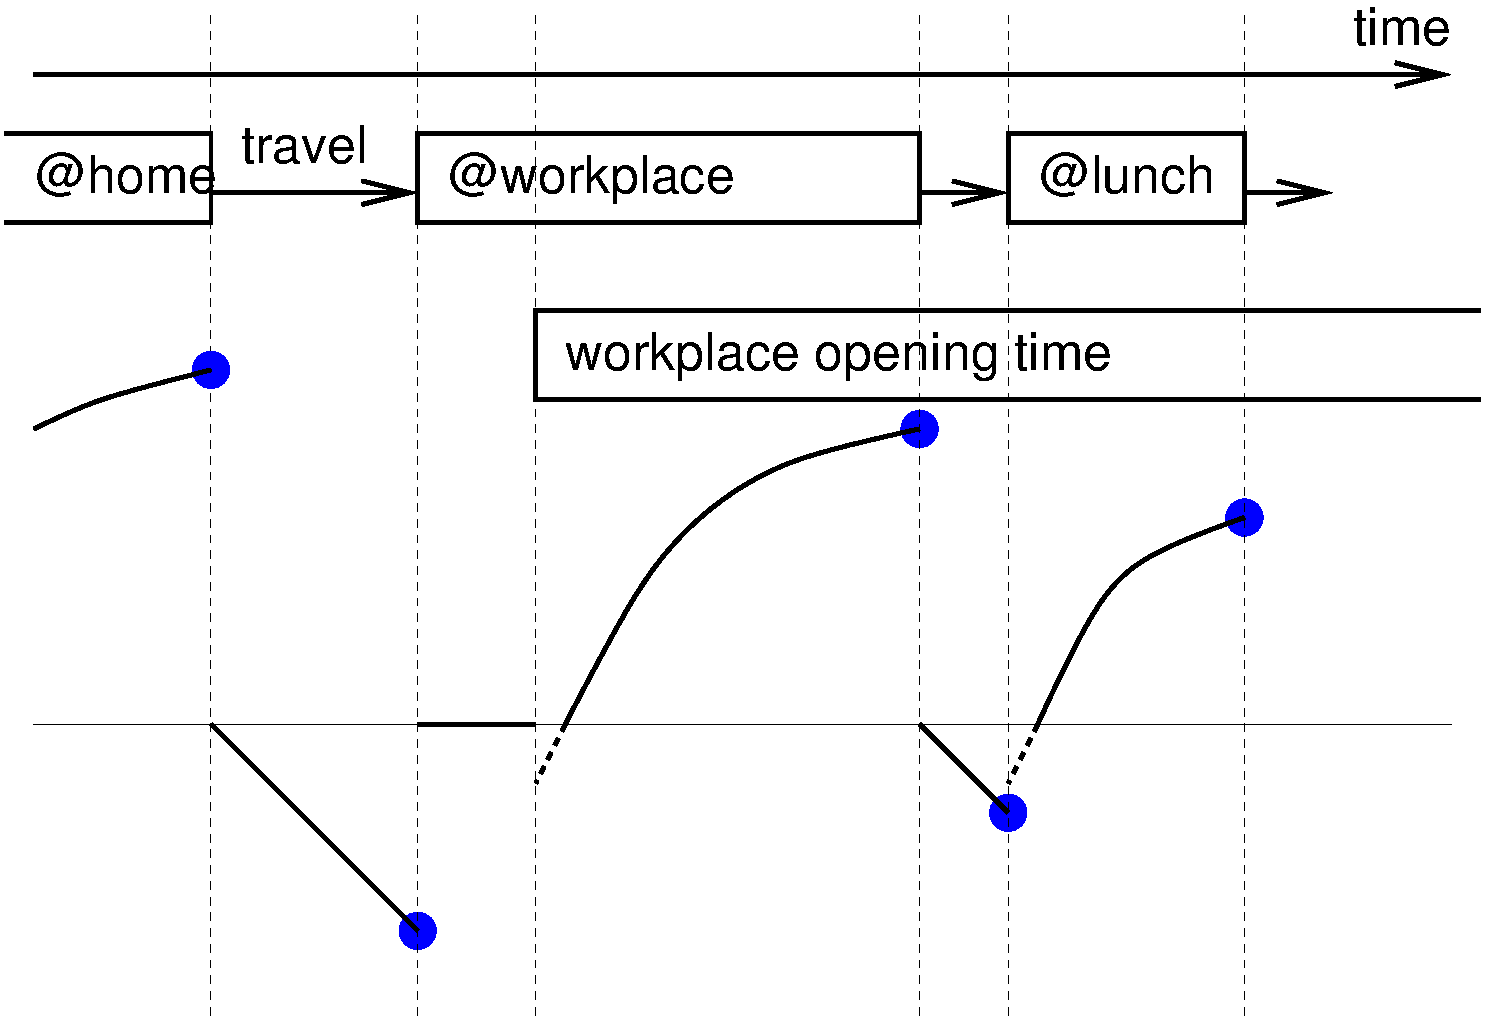
\includegraphics[width=0.6\hsize]{figures/scoringFunction/scoring-example-wo-marginal}
}
\caption{Example of scoring function.}
\label{fig:scoring-example-wo-marginal}
\end{figure}

\section{Illustration}

Synthetic travelers normally receive rewards (positive utility) for performing activities, and penalties (negative utility) for traveling.

Fig.~\ref{fig:scoring-example-wo-marginal} provides an example of a typical scoring function.  
%
Time increases to the right. 
%
The agent first is at home, then travels to the workplace, then travels to lunch, etc.
%
The workplace opening time is different from the time span during which the agent is at the workplace.
%
The distance of the blue dots to the zero line is what the synthetic persons receive at the end of each stage:
\begin{itemize}
\item a positive utility from the ``home'' activity
\item a negative utility from travelling to work
\item ``nothing'' from waiting until the workplace opens
\item a positive utility from the ``work'' activity
\item a negative utility from travelling to lunch
\item etc.
\end{itemize}

One can observe the following:
\begin{itemize}
\item extending an activity increases the utility
\item however, the \emph{marginal} increase of utility \emph{de}creases with increasing utility duration
\item ``doing nothing'' brings neither reward nor penalty
\item travelling incurrs negative utility
\end{itemize}

%% If one looks at the slopes (marginal utilities) at the actual activity durations (Fig.

%% \begin{figure}[h]
%% \centerline{%
%% 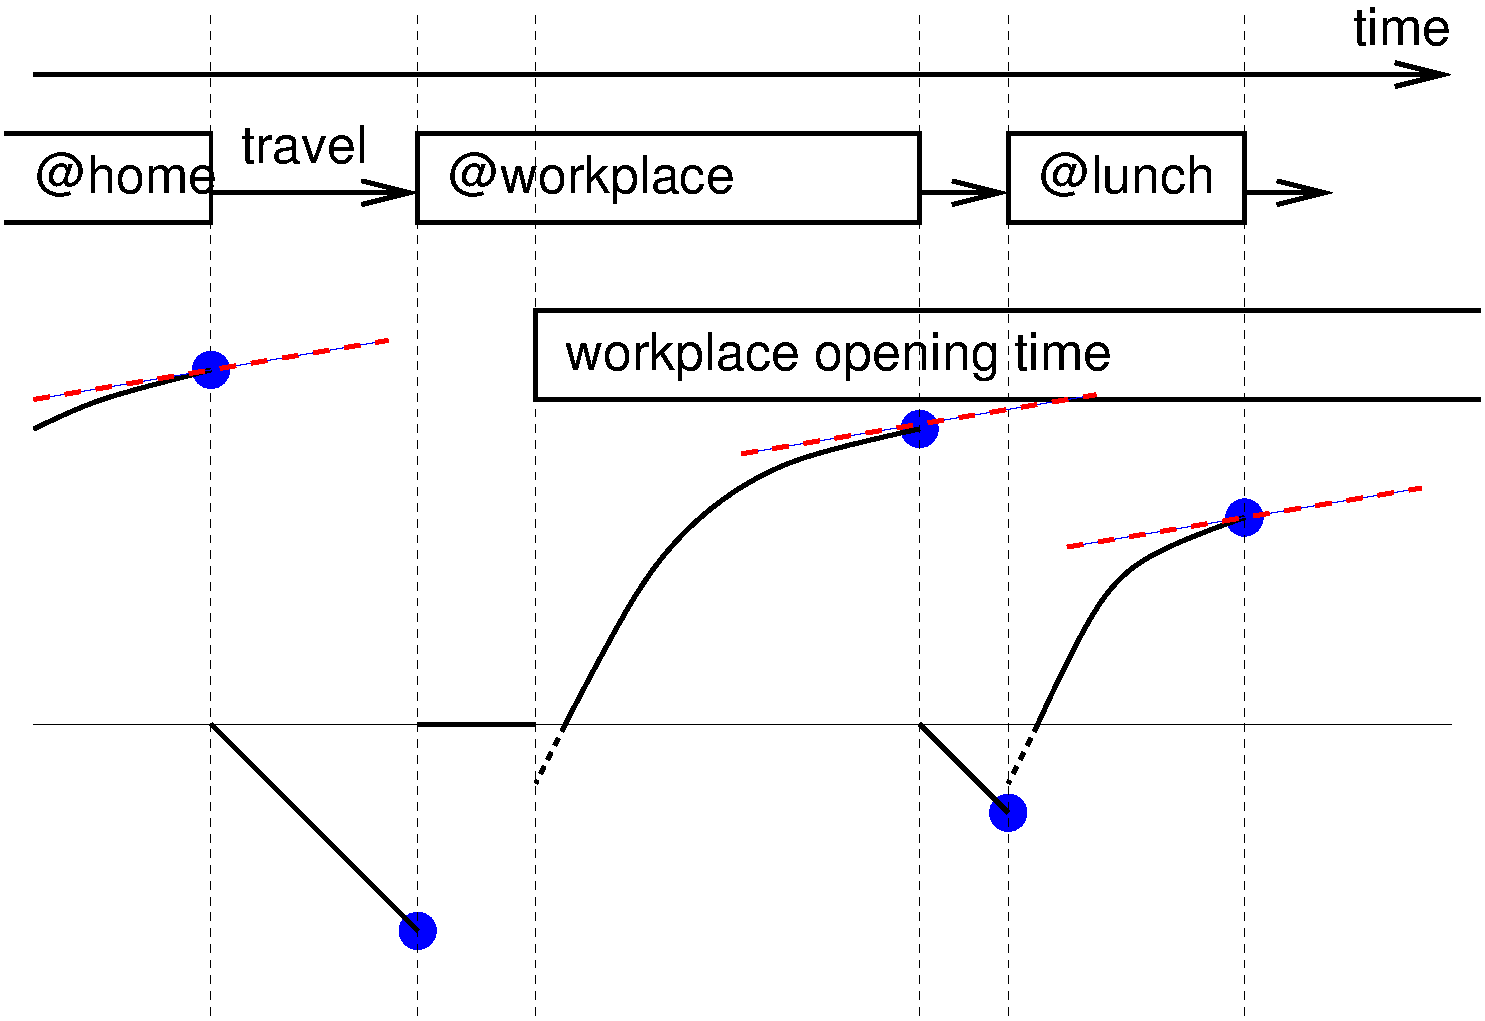
\includegraphics[width=0.6\hsize]{figures/scoringFunction/scoring-example}
%% }
%% \caption{Example of scoring function.}
%% \label{fig:scoring-example}
%% \end{figure}

\section{Mathematical version}

The mathematical version of the scoring function is
\[
V = \sum_i ( V^{perf}_i + V^{late}_i) + \sum_j V^{leg}_j \ .
\]

\subsection{Performing activities}

The (normally positive) reward of performing activity $i$ is
\[
V^{perf}_i = \beta_{perf} \cdot t_{typ,i} \cdot \ln( t_{perf} / t_{0,i} ) 
%
\qquad \mbox{ for } \qquad
%
t_{perf} \ge t_{0,i} \ ,
\]
where
\begin{itemize}

\item
$t_{perf}$ is how long the agent performed the activity, 

\item $t_{typ,i}$ is its typical duration (e.g.\ 8~hours for ``work'', 12~hours for ``home''), and

\item $\beta_{perf}$ is a slope.

\item  $t_{0,i}$ is more confusing than it looks, and has less influence than one may think, and therefore we ignore it for the time being.

\end{itemize}

\subsection{Arriving late}

The (normally negative) penalty of arriving late is
\[
V^{late}_i = \beta_{late} \cdot t_{late} \ ,
\]
where $t_{late}$ is the amount of time the agent arrived late, and $\beta_{late}$ is a (normally negative) slope.

\subsection{Traveling}

The (normally negative) penalty of traveling is
\[
V^{leg}_j = \beta_{trav,mode} \cdot t_{trav} 
%
+ \beta_m \cdot m_{trav}
%
+ (\beta_{dist,mode} + \beta_m \cdot \gamma_{dist,mode}) \cdot d_{trav}
%
+ V_{transfer}
\]
where
\begin{itemize}
\item $t_{trav}$ is the time spent traveling
\item $\beta_{trav,mode}$ is a (normally negative or zero, see below) slope
\item $m_{trav}$ is the change of the monetary position caused by the travel (normally negative, e.g.\ a toll or a fare)
\item $\beta_m$ is a (normally positive) slope; this is the marginal utility of money
\item $d_{trav}$ is the distance of the leg
\item $\beta_{dist,mode}$ is a (normally negative) slope
\item $\gamma_{dist,mode}$ is a (normally negative) distance cost rate
\item $V_{transfer}$ is a transfer penalty e.g.\ incurred in public transit systems
\end{itemize}
The negative effects of distance can be included both directly as a marginal disutility and indirectly as a distance cost rate.  The first is presumably more applicable for a mode with mostly physical exercise, such as walk, whereas the latter is presumably more applicable for a mechanical mode, such as car.  Bicycle may incur both.

The notation deliberately uses ``leg'' and not trip, since this allows to decompose a trip into multiple legs, all with separate scoring contributions.

\subsection{Utility of time as a resource (opportunity cost of time)}
\label{sec:utl-of-time-as-resource}

Most utility-based models in travel behavior research, such as typical logit mode choice models, use partial utility functions: These utility functions do not describe the full utility of the person, but just those parts that are affected by the choice.

Since MATSim gives a score/utility to the full day, this does not work in the same way any more.  It most importantly shows up with time, where reducing the time spent traveling does not only lead to a reduction of the penalty of traveling, but also (barring opening time constraints) to an extension of the activity following the travel.

The first effect is described marginally by
\[
- \frac{\partial}{\partial t_{trav}} V^{leg} = - \beta_{trav,mode} \ ,
\]
the minus stems from the fact that we are \emph{reducing} the travel time.

The second effect is described marginally by
\[
\frac{\partial}{\partial t_{perf}} V^{perf}_i
%
= \beta_{perf} \cdot t_{typ,i} \cdot \frac{1}{t_{perf}}
%
\approx \beta_{perf} \ ,
\]
where the approximation holds when the actual activity duration $t_{perf}$ is close to its typical duration, $t_{typ,i}$.  This is also the justification why $t_{typ,i}$ is called the typcical duration, and $\beta_{perf}$ the marginal utility of performing.

The marginal utility of travel time savings needs to consider both:
\[
mUTTS 
%
= \left( - \beta_{trav,mode} + \beta_{perf} \cdot \frac{t_{typ,i}}{t_{perf}} \right)
%
\approx - \beta_{trav,mode} + \beta_{perf} \ .
\]
In consequence, $\beta_{trav,mode}$ \myemph{is only an offset to the marginal utility of time as a resource}.  If travelling is considered more pleasant than ``doing nothing'', it may actually be positive.  Even when it is positive, the overall marginal utility of travel time ($= -mUTTS$) can still remain negative.

The better known (marginal) value of travel time savings is obtained by dividing these values by the marginal utility of money:
\[
VTTS = \frac{mUTTS}{\beta_m} 
%
= \frac{\left( \beta_{perf} \cdot \frac{t_{typ,i}}{t_{perf}} - \beta_{trav,mode} \right)}{\beta_m}
%
\approx \frac{\beta_{perf} - \beta_{trav,mode}}{\beta_m} \ .
\]



\section{Calibration of the scoring function}

%% \subsection{Quickstart}
\label{sec:quickstart-kn}

A possible approach is as follows:\footnote{%
%
Different groups have different systems, this is mine, although I took ideas from Michael Balmer.
%
}
\begin{enumerate}

\item Set $\beta_{scale} \equiv$ \verb$BrainExpBeta$ to $1.0$.  (This is the default.)

This is normally a positive value.

\item Set $\beta_{money} \equiv$ \verb$marginalUtilityOfMoney$ to whatever is the prefactor of your monetary term in your mode choice logit model.

If you do not have a mode choice logit model, set to $1.0$. 

This is normally a positive value (since having more money normally increases utility).

\item Set $\betaperf \equiv$ \verb$performing$ to whatever is the prefactor of car travel time in your mode choice mode (probably with a sign change, see below).

If you do not have a mode choice logit model, set to $+6.0$.

This is normally a positive value (since performing an activity for more time normally increases utility).

\item Set $\beta_{tt,car} \equiv$ \verb$traveling$ to $0.0$.

\myemph{It is important to understand this:}  Even if this value is set to zero, traveling by car will be implicitly punished by the so-called opportunity cost of time: If you are traveling by car, you cannot perform an activity, and thus you are (marginally) losing $\betaperf$.  Sometimes also called the ``utility of time as a resource''.

\item Set all other marginal utilities of travel time by mode \myemph{relative to the car value}.

E.g.\ if your logit model says something like 
\[
... -6/h \cdot tt_{car} - 7/h \cdot tt_{pt} ... ,
\]
then 
\[
\betaperf = 6 \ , \ \ \beta_{tt,car} = 0 \ , \hbox{ and } \beta_{tt,pt} = -1 \ .
\]

If you do not have a mode choice logit model, set all $\beta_{tt,mode} \equiv$ \verb$travelingXxx$ values to zero (i.e.\ same as car).

\item Set the distance cost rates \verb$monetaryDistanceCostRateXxx$ to plausible values if you have them.

For the time being, this needs to be negative (which is not entirely plausible but it is the way it is).

\item Use the alternative-specific constants $C_{mode} \equiv$ \verb$constantXxx$ to calibrate your modal split.

(This is, however, not completely simple: One needs to run iterations and look at their end, and especially for modes with small shares one needs to have innovation switched off early enough near the end of the iterations.)

\end{enumerate}

If you end up having your modal split right but its distance distribution not, you probably need to look at the different mode speeds.  In our experience this works better than using the $\beta_{tt,mode}$ for this.

Calibrating schedule-based pt currently goes beyond what can be provided here; recommendations:
\begin{itemize}

\item Stay away from schedule-based pt until you really understand what you are doing.

\item Treat schedule-based pt as a ``mechanical'' model which just transports people.  For this, completely switch off mode choice.

\item Make a support contract with senozon.

\item Write a joint funding proposal with the MATSim group in Berlin (or in Zurich, but I haven't asked them).  This needs to provide funding for us that is large enough to do research and not just support.

\end{itemize}

%% \subsection{Some explanation: Simplified version}
%% \label{sec:some-expl-simpl}

%% The simplified version assumes that all activities operate near their typical duration. In this case (see \href{http://matsim.org/node/651}{here}),  one can approximate the marginal utility of activity duration (i.e. the  marginal utility if the sum of all activities is extended by that  amount of time) by $\betaperf$.

%% Now let us consider the typical changes (of the Vickrey  scenario). Note that in the Vickrey scenario, the meaning of the  marginal utility of arriving earlier means the marginal contribution  assuming that the travel time remains the same. We will assume  that activities are ended by the endtime attribute, not by the duration  attribute.

%% \subsubsection{Travel takes longer (by amount $\Delta t$)}

%% In this situation, the activity that follows the trip is cut short by  $\Delta t$. We thus have the following (linearized) modifications  of the utility:
%% \begin{itemize}

%% \item Travel takes longer by $\Delta t$; the utility change is  $\beta_{tt} \cdot \Delta t$. Note that $\beta_{tt}$ typically is  negative.

%% \item The following activity is shortened by $\Delta t$; the (linearized)  utility change is $- \betaperf \cdot \Delta t$.  $\betaperf$ is  typically positive, so the contribution is negative.

%% \end{itemize}
%% Overall: The (linearized) utility change caused by longer travel is
%% \[
%% ( - \betaperf + \beta_{tt} ) \cdot \Delta t \ .
%% \]


%% \subsubsection{Traveller increases arriving early (by amount $\Delta t$)}

%% In this situation, the traveller will ``do nothing'' between the  arrival and the opening time of the activity. That is, the amount  of time that the traveller is doing nothing is now increased by  $\Delta t$. Consistent with the meaning of the Vickrey parameter  ``marginal utility of arriving early'', we assume that the travel time is  the same compared to the later arrival. This means that the preceeding  activity was cut shorter by $\Delta t$. We thus have the following  (linearized) modifications of the utility:
%% \begin{itemize}

%% \item The preceeding activity is shortened by $\Delta t$; the
%% (linearized) utility change is $- \betaperf \cdot \Delta t$.
%% 	$\betaperf$ is typically positive, so the contribution is
%% 	negative.

%% \end{itemize}
%% There are no other contributions, since the time between the  arrival and the opening time prodices neither positive nor negative  utility contributions. Overall: The (linearized) utility change  caused by arriving early is
%% \[
%% - \betaperf \cdot \Delta t \ .
%% \]
%% That is, as long as there are no  additional utilities or disutilities of waiting, the marginal utility of  performing can be approximated by the marginal utility of schedule  delay early.

%% \subsubsection{Traveller increases arriving late (by amount $\Delta t$)}

%% In this situation, we have the following (linearized) modifications of the utility:
%% \begin{itemize}

%% \item The preceeding activity is extended by $\Delta t$; the
%% (linearized) utility change is $\betaperf \cdot \Delta
%% t$. $\betaperf$ is typically positive, so the contribution is
%% positive.

%% \item The following activity is shortened by $\Delta t$; the (linearized)  utility change is $- \betaperf \cdot \Delta t$. $\betaperf$ is  typically positive, so the contribution is negative (and exactly cancels  the previous contribution).

%% \item Arriving late is increased by $\Delta t$; the (exact) utility change  is $\beta_{late} \cdot \Delta t$. $\beta_{late}$ is typically negative, so  the contribution is negative.

%% \end{itemize}

%% Overall: The (linearized) utility change caused by increasing the amount of arriving late is
%% \[
%% \beta_{late} \cdot \Delta t \ .
%% \]


% this is already said above (in quickstart)
%%\subsubsection{Overall}

%%Overall, calibration of the Charypar-Nagel scoring function is best done as follows:
%%\begin{itemize}
%%	\item \textbf{Run a survey and estimate logit models that include  penalties for travelling (by mode), schedule delay early, and schedule  delay late.}
%%	\item \textbf{The marginal utility of schedule delay early from the logit  model, multiplied by minus one, results in the MATSim beta\_perf.}  Since the marginal utility of schedule delay early is typically  negative, beta\_perf is thus typically positive. This is the  marginal opportunity cost of time. A useful interpretation is that  this is the difference between "leisure" and "doing nothing".
%%	\item \textbf{The marginal utility of travelling from the logit model, \emph{plus beta\_perf,} results in the MATSim beta\_trav (by mode).} That is, the MATSim beta\_trav is an \emph{additional utility offset}  when compared to doing nothing. Since driving can well be seen as  more positive than doing nothing (e.g. because of making phone calls,  listening to music, enjoying to drive), the MATSim beta\_trav can well be  positive.
%%\\   (Note that this has still nothing to do with "positive values of  travel time", e.g. by Susan Handy. Those positive values imply  that the additional utility offset over-compensates the marginal  opportunity cost of time. In other words, "time spent driving  home" is (to an extent) seen more positive than "being at home".)
%%	\item \textbf{The marginal utility of being late from the logit model results in the MATSim beta\_late.}
%%	\item Note that you also need reasonable values for opening time, latest  arrival time, and closing time, in order to achieve that the schedule  delay cost mechanics works in MATSim. This is quite clear if you  think about it; nevertheless, it has been forgotten uncountable times  (in particular in studies that start from trips, not from full daily  plans).
%%\end{itemize}

%% \subsection{Without schedule delay}

%% If you intend to run MATSim without time adaptation  (TimeAllocationMutator), these things are not that critical. In  that situation, you just need to make sure that $\betaperf + \beta_{tt}$  matches your marginal utility of travel time savings. An easy  way in our view is:
%% \begin{itemize}

%% \item Set $\beta_{tt,car}$ to zero (i.e.\ assume that driving
%% 	is as good or bad as doing nothing).  

%% \item Set $\betaperf$ to
%% 	the estimated marginal utility of travel time savings (make
%% 	sure you get the sign right; $\betaperf$ should be
%% 	positive).  \item Set (say) $\beta_{tt,pt}$ to your estimated
%% 	marginal utility of travel time savings (should be
%% 	positive) \emph{minus} the MATSim $\betaperf$. The result may
%% 	be positive (implying that spending time using the mode is
%% 	better than doing nothing) or negative (implying that spending
%% 	time using the mode is worse than doing nothing).
%% \end{itemize}
%% Note that even without time adaptation, $\beta_{late}$ may still have an influence if you have set the latest arrival times for some  activities.

%% \subsection{Full version}

%% ``Full version'' would imply that we could calibrate the MATSim  parameters also for situations where the actual activity durations are  far from their ``typical'' values. This could happen for two reaons:
%% \begin{itemize}

%% \item There are too many activities that need to be squeezed into a  day. A possible interpretation would be that $\betaperf$ corresponds  to the marginal utility of additional leisure time on, say, sundays,  but the weekday activites cannot be shifted to sundays.

%% \item There are too many activities that need to be squeezed
%% into certain time periods, say between day care opening and closing,
%% or into typical business hours.

%% \end{itemize}
%% Both of these interpretations make sense (in my view) and should be
%% investigated for MATSim. Presumably, there is already general
%% research; it would then be necessary to bring that research and the
%% MATSim formulation together.


\section{Default values for the Charypar-Nagel scoring function}

As explained \href{http://matsim.org/node/650}{here},  the MATSim scoring function has, under some circumstances (actual  durations near "typical" durations"), some similarity to the Vickrey  scenario.

The "typical" parameters of the Vickrey scenario are 
\[
\hat\beta_{early}=-6~,~~\hat\beta_{travel}=-12~\mbox{, and } \hat\beta_{late}=-18 \ .
\]

For MATSim, as explained in Sec.~\ref{sec:utl-of-time-as-resource}, %Sec.~\ref{sec:some-expl-simpl}, 
this translates into
\[
\betaperf=6~,~~\beta_{travel}=-6\mbox{ , and } \beta_{late}=-18 \ . 
\]
These are the parameters that were, for a lack of  estimated parameters, introduced into (the precursor of) MATSim  approximately in 2006.

These parameters are multiplied with the beta\_brain parameter, which  can be seen as a separately configurable logit scale parameter. A  useful setting for this parameter was determined via systematic tests  concerning the stability of the iterations, see \href{https://svn.vsp.tu-berlin.de/repos/public-svn/publications/vspwp/2004/04-03/}{here}.

As a next step, an infrastructure to compare MATSim simulations with  real world traffic counts was set up. Only after that  infrastructure was there, an attempt to calibrate the MATSim parameters  from a survey was made. This is documented \href{https://svn.vsp.tu-berlin.de/repos/public-svn/publications/vspwp/2009/09-10/}{here}, unfortunately in German. Two results were
\begin{itemize}
	\item The estimated parameters all have the same order of magnitude as the MATSim default parameters (the "Vickrey" parameters).
	\item The results with respect to traffic counts were not considerably different from before.
\end{itemize}



\section{Interpretation of the logarithmic "utility of performing"}

The  so-called "Charypar-Nagel scoring function" is used in many  MATSim  studies. It is called that way because there is an ancient paper   where this scoring function was introduced.

It uses a logarithmic utility of time for activities: $U = \beta \cdot t_{typ} \cdot  \ln(x/t_0)$ . I sometimes call $t_{typ}$ the ``typical duration''.

The first derivative of U is beta at the typical duration:
\begin{itemize}
	\item 
$\displaystyle
\frac{dU}{dx} = \beta \cdot t_{typ} / x
$
	\item 
$\displaystyle
\left. \frac{dU}{dx}\right|_{x=t_{typ}} = \beta
$
\end{itemize}

Interpretation: marginal utility of duration at "typical duration" is indep of activity type. (*)

The second derivative of U at the typical duration is
\begin{itemize}
	\item 
$\displaystyle
\frac{d^2U}{dx^2} = - \beta \cdot t_{typ} / x^2
$
	\item 
$\displaystyle
\left. \frac{d^2U}{dx^2} \right|_{x=t_{typ}} = - \beta / t_{typ}
$
\end{itemize}

An  important consequence of this is that there is no separate  free  parameter to calibrate the curvature (= 2nd derivative) at the  typical  duration: $\beta$ needs to be the same across all activities, and  $t_{typ}$ is  given by (*).

A second consequence is that $t_0$ is largely  irrelevant. It  shifts the function up and down, i.e.\ it determines how  much you lose  if you drop an activity completely.

In the  original paper (and in most of MATSim), $t_0$ is set to $t_{typ} \cdot   \exp(-10h/t_{typ})$ . This has the (intended) consequence that all  activities  have the same utility contribution at their typical  duration:
\[
U = \beta \cdot t_{typ} \cdot \ln( x / t_{typ} / \exp(-10h/t_{typ}) ) 
%
= \beta \cdot t_{typ} \cdot [ \ln( x/t_{typ} ) + 10h/t_{typ} ]
\]
which   is, at $x=t_{typ}$,
\[
= \beta \cdot t_{typ} \cdot [ 0 + 10h/t_{typ} ] = \beta \cdot  10h \ . 
\]
With  our usual $\beta = 6Eu/h$, this results in $60Eu$ per  activity.

The slope at $U=0$, i.e.\ at $x=t_0$, is
\[
(\beta \cdot t_{typ} / t_{typ}) \cdot \exp( 10h/t_{typ}) = \beta \cdot \exp( 10h/t_{typ} )
\]
which \emph{de}creases with increasing $t_{typ}$. This means that activities with larger typical duration are \emph{easier} to drop completely.

In the end, this makes sense: Since the additional score of any activity is the same, the score \emph{per time} is smallest for activities with long typical durations. Therefore, it makes sense to drop them first.

But practically, this is probably not desired behavior, since it would first drop the home activity from a daily plan.

Overall, therefore: \myemph{In my opinion, the current utility function does not work for activity dropping.}

---

An  alternative, never tested since activity dropping was never  tested with  this utl fct, would be to recognize that $U'(t_0) = \beta \cdot  t_{typ} / t_0$ ,  i.e.\ \emph{increasing} \emph{slope} with \emph{decreasing}  $t_0$.  That is, high priority activities should have $t_0$ such that  $t_{typ}/t_0$ is  large (large slope = hard to drop). Activities of the  same priority  should have $t_0$ such that $t_{typ}/t_0$ is the same between  those activities.  Overall, something like
\[
weight \propto t_{typ}/t_0
\]
or
\[
t_0 \propto t_{typ}/weight
\]
where large weight implies a large importance of the activity.

This  was, as said, never tried, since activity dropping was never   systematically tried. It also does not fix the problem, discussed   later, that different activities might have different resistance  against  making them shorter; since this is U'', this is -beta/t\_x  with the  above utl fct: activities are shortened proportional to their  typical  duration.

---

\st{To make matters worse, there is currently the  convention that  negative values of U are set to zero. This is done  since we need  useable values for negative durations (since they may  happen at the  "stitching together" of the last to the first activity of a  day), and  if we give those a "very negative" score, then the utl at t=0  cannot be  even smaller than this.}

\st{This has, however, the  unfortunate consequence that the ``drift  direction'' of the adaptive  algorithm, once an activity duration has  gone below $t_0$, goes to zero  duration.}

The above was modified in nov'13, see \url{https://matsim.atlassian.net/browse/MATSIM-191}.  It now takes the slope at $t=t_0$ and extends it with that slope to the left.

\section{Outlook}

Outlook: What would we want for our next generation utl function? Some wishes from my perspective:
\begin{itemize}
	\item Curvature at typical duration can be calibrated
	\item Slope at $U=0$ can be calibrated
	\item Utl function extends in meaningful way to negative durations (this would fix the arbitrary handling that we currently employ)
\end{itemize}

In  my view, a polynomial of second degree would be worth trying.\footnote{%
%
As  usual,  there are several ways to set this up. One way is to  expand around the  typical duration:
\[
U(t_{typ} + \epsilon) = U(t_{typ}) + \epsilon \cdot U'(t_{typ}) + \epsilon^2 * U''(t_{typ})/2
\]
or
\[
U(x) = U(t_{typ}) + (x-t_{typ}) \cdot U'(t_{typ}) + (x-t_{typ})^2 * U''(t_{typ})/2
\]
with $t_{typ} =$ typical duration, $U'(t_{typ}) = \beta =$ marg utl at typ dur, $U''(t_{typ}) =$  curvature at typ dur (``priority''), and $U(t\_x) =$ ``base value of act'' (which could be something like $\beta \cdot t_{typ}$ ).
\\
---
\\
Another way (having the parabola going through (0,0)) would be
\[
U(x) = - a x ( x - c ) = - a x^2 + a c x
\]
\[
U'(x) = - 2 a x + a c
\]
\[
prio = U'(x=0) = a c , i.e.\ c = prio/a .
\]
\[
\beta = U'(x=t_{typ}) = - 2 a t_{typ} + prio \hbox{, i.e.\ } a = (prio - \beta)/2t_{typ}
\]
}

There is other work (e.g. by Joh) that should be looked at.

% Local Variables:
% mode: latex
% mode: reftex
% mode: visual-line
% TeX-master: "../user-guide.tex"
% comment-padding: 1
% fill-column: 9999
% End: 

\NextFile{StrategyModules.html}
\chapter{Strategy Modules}

\authorsOfDoc{Kai Nagel}

\bigskip

\begin{chapter-intro}
Strategies describe how agent plans' are modified and are thus an important
part of MATSim's evolutionary optimization algorithm. 
\end{chapter-intro}


\section{Introduction}
\label{sec:introduction}


Strategy Modules can be configured in the configuration file via the following syntax:
\begin{lstlisting}{language=XML}
<module name="strategy" >
    <param name="ModuleProbability_1" value="0.1" />
    <param name="Module_1" value="ChangeLegMode" />
    <param name="ModuleProbability_2" value="0.1" />
    <param name="Module_2" value="TimeAllocationMutator" />
</module>
\end{lstlisting}

In the configuration file, strategy modules are numbered. Also, each module is given a weight 
which determines the probability by which the course of action represented by the module is taken. 
In this example, each person stands a chance of 1/2 that their transport mode is changed,  and a chance of 1/2 that their time allocation is changed. (The  weights are renormalized so that they add up to one.)

A strategy module is, in the code, always a combination of a plan  selector and zero or more strategy module elements. There are two cases,  which are handled differently:
\begin{itemize}
	\item If there are zero strategy module elements, the chosen plan is made "selected" for the person, and the method returns.
	\item If there is at least one strategy module element, the chosen plan is  copied, that copy is added to the persons's set of plan, and the new  plan is made "selected". That new plan is then given to the  strategy module elements for modification. These latter strategy  modules, with at least one strategy module element, are sometimes called  "innovative".
\end{itemize}

The strategy modules that are understood by MATSim are defined in the class \href{http://www.matsim.org/xref/org/matsim/core/controler/PlanStrategyRegistrar.html}{PlanStrategyRegistrar}. In addition, you can program your own strategy modules; see tutorial.programming in matsim/src/main/java for examples.

Unfortunately, the naming in the code is different from the naming in the config file:
\begin{itemize}
	\item "strategy" in config file $\rightarrow$ StrategyManager (or "set of strategies") in code
	\item "strategy module" in config file $\rightarrow$ PlanStrategy in code
	\item There is a PlanStrategyModule in the code; it corresponds to what was called strategy module element in the description above.
\end{itemize}

It is not clear which combinations of these modules can be used  together. Depending on required features, special variants sometimes  need to be used. This has not yet been sorted out. Also see \href{http://matsim.org/node/690}{here}.


\umbruch

\section{Selectors}
\label{sec:selectors}

Selectors are pure plan selecting (i.e.\ non-innovative) strategy module.

\subsection{BestScore.  Status: works}

Will select the plan with the highest score. The score will be updated after execution of the mobsim.

Disadvantage: Will never try again plans that obtained a bad score  from a fluctuation (e.g.\ a rare traffic jam). It is therefore  recommended to either use this in conjunction with a small probability  for RandomPlanSelector, or to use ChangeExpBeta.

\subsection{ChangeExpBeta. Status: works. RECOMMENDED!}

Choice model between plans that \emph{converges} to a logit distribution.

The scores $S_i$ are taken as utilities; the betaBrain parameter from the  config file is taken as the scale parameter. As equation:
\[
p_i = \frac{\exp( \beta_{brain} * S_i)}{\sum_j \exp( \beta_{brain} * S_j )} \ .
\]

\subsection{KeepLastSelected. Status: works}

Pure plan selecting (i.e.\ non-innovative) strategy module.

Will keep the selected plan selected.  This may be necessary since \emph{every} person will have to undergo plans selection.

\subsection{SelectExpBeta. Status: works}

Multinomial logit model choice between plans.

The scores $S_i$ are taken as utilities; the betaBrain parameter from the  config file is taken as the scale parameter. As equation:
\[
p_i = \frac{\exp( \beta_{brain} * S_i)}{\sum_j \exp( \beta_{brain} * S_j )} \ .
\]

\subsection{SelectRandom.  Status: works}

Pure plan selecting (i.e.\ non-innovative) strategy module.

Will select a random plan.

\umbruch
\section{Innovative modules}

Sec.~\ref{sec:selectors} was about strategy modules which would just select between plans.

This section is about innovative modules which modify plans.

Note that innovative modules first copy a plan and then modify it, i.e.\ they increase the choice set.  Pure selectors do not do this.

\subsection{ReRoute.  Status: nearly indispensable}

\maintainers{Marcel Rieser, Thibaut Dubernet}

All routes of a plan are recomputed.

The module is called by inserting the following lines into the "strategy" module:
\begin{lstlisting}{language=XML}
<module name="strategy" >
    <param name="ModuleProbability_XXX" value="0.1" />
    <param name="Module_XXX" value="ReRoute" />
    ...
</module>
\end{lstlisting}


The corresponding configuration module unfortunately has a different name:
\begin{lstlisting}{language=XML}
<module name="planscalcroute" >
    <param name="beelineDistanceFactor" value="1.3" />
    <param name="bikeSpeed" value="4.166666666666667" />
    <param name="ptSpeedFactor" value="2.0" />
    <param name="undefinedModeSpeed" value="13.88888888888889" />
    <param name="walkSpeed" value="0.8333333333333333" />
</module>
\end{lstlisting}

This works pretty reliably for car.

It also works for other modes, as "pseudo"-mode, in the following way:
\begin{itemize}
	\item Travel times for these other modes are not obtained from true  routing on the corresponding network, but by some estimates. These  are configured by the parameters above, but no guarantee that they work  consistently.
	\item The mobsim will not execute such routes on the network, but "teleport" them.
	\item The scoring works quite normally, since it just takes the time from leg start to leg end by mode.
\end{itemize}

It is possible to route such legs on the network, by using a different router.

It is \emph{not} possible to "physically" execute a leg in the  mobsim if it has not been routed before. That is, the capability  of the router needs to be $\ge$ the capability of the mobsim.  (Makes sense, if one thinks about it.)

\subsection{TimeAllocationMutator.  Status: works}

Simple  module that shifts activity end times randomly. ("Good" time  shifts will be selected through the matsim plans selection mechanism.)

The maximum extent of the shifts can be configured; see the config  section of the log file. 
%%It is, as of now (may'10), not possible  to add a comment to that parameter.
% I think this has now been working for a long time, by making this a core config group. kai, oct'13

The usage of the module is configured in the ``strategy'' section.

\subsection{ChangeSingleLegMode. Status: works}

\maintainers{Marcel Rieser}

This replanning module randomly picks one of the plans of a person and changes the mode of transport of \textbf{one single leg}. The leg is picked randomly. For changing the mode of transport for all legs use \verb$ChangeLegMode$ (Sec.~\ref{sec:changeLegMode}). In contrast to \verb$ChangeLegMode$,  \verb$ChangeSingleLegMode$ allows for multiple modes in one plan. By default,  the supported modes are driving a car and using public transport. Also,  this module is able to (optionally) respect car-availability.

Note that the configuration is done by \verb$<module name="changeLegMode">$ and not by \verb$<module name="changeSingleLegMode">$. The replanning module is configured like  this using the very same configuration module as \verb$ChangeLegMode$:
\begin{lstlisting}{language=XML}
<module name="changeLegMode">
    <param name="modes" value="car,pt,bike,walk" />
    <param name="ignoreCarAvailability" value="false" />
</module>
\end{lstlisting}

Add the module to the replanning strategy like this:
\begin{lstlisting}{language=XML}
<param name="Module_X" value="ChangeSingleLegMode" />
<param name="ModuleProbability_X" value="0.1" />
\end{lstlisting}

Replace the 'X' with the number you assign to this module. For some more details on the syntax of this section, see Sec.~\ref{sec:introduction}.

By default, the simulation will handle legs with modes different from  ``car'' by using a delayed teleportation. If another behavior is  requested (e.g.\ detailed simulation of public transport), this needs to  be manually configured for the simulation.


\subsection{ChangeLegMode. Status: works}
\label{sec:changeLegMode}

\maintainers{Michael Zilske}

This replanning module randomly picks one of the plans of a person  and changes its mode of transport. By default, the supported modes  are driving a car and using public transport. Only one mode of transport  per plan is supported. For using different modes for sub-tours on a  single day see the "SubtourModeChoice" module. Also, this module is able  to (optionally) respect car-availability.

The replanning module is configured like this, where the value  parameter lists the modes of transport from which the module randomly  chooses:
\begin{lstlisting}{language=XML}
<module name="changeLegMode">
    <param name="modes" value="car,pt,bike,walk" />
    <param name="ignoreCarAvailability" value="false" />
</module>
\end{lstlisting}

Add the module to the replanning strategy like this:
\begin{lstlisting}{language=XML}
<param name="Module_X" value="ChangeLegMode" />
<param name="ModuleProbability_X" value="0.1" />
\end{lstlisting}

Replace the 'X' with the number you assign to this module. For some more details on the syntax of this section, see \href{http://matsim.org/node/478}{here}.

By default, the simulation will handle legs with modes different from  "car" by using a delayed teleportation. If another behavior is  requested (e.g.\ detailed simulation of public transport), this needs to  be manually configured for the simulation.

This module can be used with the detailed simulation of public transport by changing the line

\begin{lstlisting}{language=XML}
<param name="Module_X" value="ChangeLegMode" />
\end{lstlisting}

to

\begin{lstlisting}{language=XML}
<param name="Module_X" value="TransitChangeLegMode" />
\end{lstlisting}

\subsubsection{Reference}

M. Rieser, D. Grether, K. Nagel;\textbf{Adding mode choice to a multi-agent transport simulation}; TRB'09

%%%%%%%%%%%%%%%%%%%%%%%%%%%%%%%%%%%%%%%%%%%%
%%%%%%%%%%%%%%%%%%%%%%%%%%%%%%%%%%%%%%%%%%%%
\subsection{SubtourModeChoice. Status: probably works}

\maintainers{Michael Zilske}

In contrast to "ChangeLegMode", which changes \emph{all} legs of a plan to a different mode, this module changes the modes of sub-tours separately.

For example, somebody might take the car to work, walk to lunch and back, and take the car back home.

"chainBasedModes" means modes where a vehicle (car, bicycle,  ...) is parked and in consequence needs to be picked up again.
\begin{lstlisting}{language=XML}
<module name="subtourModeChoice" >
    <param name="chainBasedModes" value="car, bike" />
    <param name="modes" value="car, bike, pt, walk" />
</module>
\end{lstlisting}


The module is called by inserting the following lines into the "strategy" module:
\begin{lstlisting}{language=XML}
<module name="strategy" >
    <param name="ModuleProbability_XXX" value="0.1" />
    <param name="Module_XXX" value="SubtourModeChoice" />
    ...
</module>
\end{lstlisting}


For modes other than car, travel time and travel distance are  computed according to some heuristics, which are configured in the  router.

\umbruch
%%%%%%%%%%%%%%%%%%%%%%%%%%%%%%%%%%%%%%%%%%%%
%%%%%%%%%%%%%%%%%%%%%%%%%%%%%%%%%%%%%%%%%%%%
% after the cleaning up of the strategies, the following seems to be so obsolet that it feels better to not show it at all. kai, oct'13

%%\section{Combination of strategy modules}

%%It  is not clear which combinations of these modules can be used together.  Depending on required features, special variants sometimes need to be  used. This has not yet been sorted out.

%%The following table tries to give an overview, but it is an old table  that has not been maintained (table status 2011; this sentence written  2012).
%%\begin{center}
%%\begin{tabularx}{\hsize}{|X|l|l|X|}
%%\hline 
%%\textbf{Choice dimension} & \textbf{Default Strategy} & \textbf{Transit} & \textbf{Transit \& Parking} \\ 
%%\hline
%%departure time choice & TimeAllocationMutator & TransitTimeAllocationMutator & ? \\ 
%%\hline
%%route choice & ReRoute & ReRoute & ? \\ 
%%\hline
%%mode choice (all legs get same mode) & ChangeLegMode & TransitChangeLegMode & ? \\ 
%%\hline
%%mode choice (each leg can have a different mode) & ChangeSingleLegMode & TransitChangeSingleLegMode & ? \\ 
%%\hline
%%mode choice (subtour-based) & SubtourModeChoice & TransitSubtourModeChoice & ? \\ 
%%\hline
%%location choice & LocationChoice & ? & ? \\ 
%%\hline
%%\end{tabularx}
%%\end{center}

%%Legend:
%%\begin{itemize}
%%	\item n/a means this choice dimension is not supported/available for the specified feature
%%	\item ? means there is no known implementation available
%%\end{itemize}
%%%%%%%%%%%%%%%%%%%%%%%%%%%%%%%%%%%%%%%%%%%%
%%%%%%%%%%%%%%%%%%%%%%%%%%%%%%%%%%%%%%%%%%%%

% Local Variables:
% mode: latex
% mode: reftex
% mode: visual-line
% TeX-master: "../user-guide.tex"
% comment-padding: 1
% fill-column: 9999
% End: 

\NextFile{OtherModules.html}
\chapter{MATSim input data (``MATSim containers'')}

Sorted alphabetically.

%%%%%%%%%%%%%%%%%%%%%%%%%%%%%%%%%%%%%%%%%%%%
%%%%%%%%%%%%%%%%%%%%%%%%%%%%%%%%%%%%%%%%%%%%
\section{"counts". Status: works for vsp and ivt}

\subsubsection{\textbf{Maintenance and Questions:}}

A. Horni, IVT (horni\_at\_IVT.baug.ethz.ch)

\subsubsection{\textbf{\textbf{Javadoc:
\\}}}

\href{http://www.matsim.org/javadoc/org/matsim/counts/package-summary.html}{www.matsim.org/javadoc/org/matsim/counts/package-summary.html}


\subsubsection{\textbf{\textbf{Config Parameters{}}}}

\href{http://www.matsim.org/javadoc/org/matsim/counts/package-summary.html#counts_parameters}{www.matsim.org/javadoc/org/matsim/counts/package-summary.html\#counts\_parameters}

\subsubsection{\textbf{In Brief:}}

MATSim can compare the simulated traffic volumes to traffic counts from the real world. Counts is the module that allows to
\begin{itemize}
	\item read some external file with traffic flow counts
	\item compare them automatically to the counts generated inside the matsim simulation
	\item submit the result to a kmz file which can be displayed inside google earth
\end{itemize}

There is a feature to re-scale the counts before comparison (for example if you are running the simulations with a 10\% sample).

\subsubsection{Comparison Data}

Prepare a file containing the real-world traffic counts. The file, e.g. named counts.xml, must follow the xml-format defined in \href{http://matsim.org/files/dtd/counts_v1.xsd}{counts\_v1.xsd}. An example of such a file can be found in MATSim at \href{http://matsim.svn.sourceforge.net/viewvc/matsim/matsim/trunk/examples/equil/counts100.xml?content-type=text%2Fplain}{examples/equil/counts100.xml}.

The file contains the following information:
\begin{itemize}
	\item For each link in the network for which traffic count information  is available, a count-element must exist. The count-element specifies  the link it refers to in its attribute 
\texttt{loc\_id}. In addition, an optional 
\texttt{cs\_id}  can be stored that may, for example, refer to the original id of the  counting station (for tracking back the origin of the data).
	\item In each count-element, 1 to 24 volume-elements can appear. Each volume-element contains the measured traffic count (attribute "
\texttt{val}") for an hour of the day (attribute "
\texttt{h}",  numbered from 1 to 24; 1 = 00:00-00:59, 2 = 01:00-01:59, etc). It is  not necessary that traffic counts are available for all 24 hours of a  day.
\end{itemize}


\subsubsection{Enabling Comparison in Configuration File}

Add the following lines to your configuration file:
\begin{lstlisting}
<module name="counts">
  <param name="inputCountsFile" value="/path/to/counts.xml" />
  <param name="outputformat" value="txt,html,kml" />
</module>

\end{lstlisting}

The comparison is automatically generated every 10th iteration.  Generated output is located in the output-directory of the iteration  (usually something like
\texttt{output/ITERS/it.10/}).


\subsubsection{Configuring the Counts Comparison}

The counts-module offers the following config-parameters:
\begin{itemize}
	\item 
\texttt{<param name="outputformat" value="txt,html,kml" />}
\\     The output format specifies in which format the comparison results are written to disk. It can be any combination of 
\texttt{txt}, html and 
\texttt{kml}. Multiple formats can be specified separated by commas. 
\texttt{txt} writes simple text-tables containing the values to a file. It is most useful to create custom graphs, e.g. in Excel. 
\texttt{html} creates a directory containing several html files, allowing to browse the results interactively. 
\texttt{kml} creates a file to be displayed in Google Earth. This last option only works if the \href{http://www.matsim.org/node/405}{correct coordinate system is set}.
	\item 
\texttt{<param name="countsScaleFactor" value="1.0" />}
\\     If you only simulate a sample of your population, the simulated  traffic volumes are likely lower than the real-world traffic counts. In  order to allow useful comparison, one can specify a factor by which the  simulated traffic volumes are multiplied. For example, if you simulate a  25\% sample of your full population, specify a countsScaleFactor  of 4.
	\item 
\texttt{<param name="distanceFilterCenterNode" value="2386" />
\\     <param name="distanceFiler" value="30000.0" />}
\\     If the traffic counts cover a larger area than the area being  simulated, the traffic counts outside your area will result in a bad  comparison. Instead of removing the traffic counts from the counts.xml,  you can specify a filter to only include some traffic counts from the  file in the comparison. To activate the filter, specify the id of a node  that acts as the center of a circle. The circle has the radius  specified in "
\texttt{distanceFilter}", the unit being the same unit as the length of links (i.e. usually meters).
\end{itemize}



\umbruch
%%%%%%%%%%%%%%%%%%%%%%%%%%%%%%%%%%%%%%%%%%%%
%%%%%%%%%%%%%%%%%%%%%%%%%%%%%%%%%%%%%%%%%%%%
\section{"facilities". Status: "user" version work in progress}

\textbf{Maintainer:} Andreas Horni

One may, or may not, use a separate file that contains "facilities" – essentially some kind of land use information.

The prototype for this is fairly old. But the final design is  somewhat different, and has not been fully executed. So I (kn) do  not know if this can currently be used as a non-developer.

\umbruch
%%%%%%%%%%%%%%%%%%%%%%%%%%%%%%%%%%%%%%%%%%%%
%%%%%%%%%%%%%%%%%%%%%%%%%%%%%%%%%%%%%%%%%%%%
\section{"households". Status: probably ready but nowhere used}

\textbf{Maintainer:} Christoph Dobler

An option to read a households file into matsim.

I (kn) don't know the exact status.

\umbruch
%%%%%%%%%%%%%%%%%%%%%%%%%%%%%%%%%%%%%%%%%%%%
%%%%%%%%%%%%%%%%%%%%%%%%%%%%%%%%%%%%%%%%%%%%
\section{"network". Status: ok}

\umbruch
%%%%%%%%%%%%%%%%%%%%%%%%%%%%%%%%%%%%%%%%%%%%
%%%%%%%%%%%%%%%%%%%%%%%%%%%%%%%%%%%%%%%%%%%%
\section{"network" (time dependent). Status: works for vsp}

\textbf{Maintenance:} G. Lämmel, VSP

MATSim provides the opportunity to model time dependent aspects of  the network explicitly. For each link in the network basic parameters  (i.e. freespeed, number of lanes and flow capacity) can be varied over  the time. So it is possible to model accidents or the like. One  particular area for this technique is the modeling of evacuation  scenarios.
In the case of an evacuation simulation the network has time dependent  attributes. For instance, large-scale inundations or conflagrations do  not cover all the endangered area at once.
In MATSim this time varying aspects are modeled as network change  events. A network change event modifies parameters of links in the  network at predefined time steps. The network change events have to be  provided in a XML file to MATSim.

A sample network change event XML file could look like:

\begin{lstlisting}{language=XML}
<?xml version="1.0" encoding="UTF-8"?>
<networkChangeEvents xmlns="http://www.matsim.org/files/dtd"  xmlns:xsi="http://www.w3.org/2001/XMLSchema-instance"  xsi:schemaLocation="http://www.matsim.org/files/dtd  http://www.matsim.org/files/dtd/networkChangeEvents.xsd">}

  <networkChangeEvent startTime="03:06:00">
    <link refId="12487"/>
    <link refId="12489"/>
    <link refId="12491"/>
    <freespeed type="absolute" value="0.0"/>
  </networkChangeEvent>

</networkChangeEvents>
\end{lstlisting}

This change event would set the freespeed of the links 
\texttt{12487, 12489, 12491} to 0 m/s at 
\texttt{03:06}  am (all values have to be provided in SI units). These values are valid  until the next network change event (if there is any) changes the  freespeed of link 
\texttt{12487, 12489, 12491} again. In this example the freespeed would be set to an absolute value. It is also possible to take the old 
\texttt{freespeed} value and multiply it by a factor. For dividing the old 
\texttt{freespeed} value by 2, the corresponding line of the network change event XML file would look like:
\\   
\texttt{<freespeed type="scaleFactor" value="0.5"/>}
\\  Besides changing the 
\texttt{freespeed}, one could also change the number of 
\texttt{lane}s:
\\   
\texttt{<lane type="absolute" value="2.0"/>}
\\  Or the flow capacity:
\\   
\texttt{<flowCapacity type="absolute" value="0.0"/>}
\\
\\  To make use of the network change events one has to define it in the  MATSim config file. Therefore the following two lines have to be added  in the network section of the config file:
\\
\texttt{<param name="timeVariantNetwork" value="true" />
\\  <param name="inputChangeEventsFile" value="path\_to\_ change\_events\_file" />}
\\
\\  Now one has just to start the controller with this config file and the network change events will be applied automatically.

It  seems that the ``absolute'' version of this module was never tested (and  may not work) with freespeeds other than zero. kai, oct'10



\umbruch
%%%%%%%%%%%%%%%%%%%%%%%%%%%%%%%%%%%%%%%%%%%%
%%%%%%%%%%%%%%%%%%%%%%%%%%%%%%%%%%%%%%%%%%%%
\section{"vehicles". Status: probably reads the file correctly, but does nothing else}

\textbf{Maintainer:} Michael Zilske (within limits of DFG/MUC project; possibly pt project)

\umbruch
%%%%%%%%%%%%%%%%%%%%%%%%%%%%%%%%%%%%%%%%%%%%
%%%%%%%%%%%%%%%%%%%%%%%%%%%%%%%%%%%%%%%%%%%%
%%%%%%%%%%%%%%%%%%%%%%%%%%%%%%%%%%%%%%%%%%%%
%%%%%%%%%%%%%%%%%%%%%%%%%%%%%%%%%%%%%%%%%%%%
\chapter{Synthetic realities (aka ``mobsims'')}

This chapter is partially deprecated, e.g.:
\begin{itemize}
\item
``qsim'' is now the default mobsim; the others need to be specifically
called for in the \verb$controler$ section of the config file.  It is also the most used and therefore probably the most reliable of the three variants.
\end{itemize}


%%%%%%%%%%%%%%%%%%%%%%%%%%%%%%%%%%%%%%%%%%%%
\section{"qsim". Status: works}

\sout{If you do \textbf{\emph{not}} put a "qsim" section into the config file, the system will use the default "simulation" (look there).}

\sout{"qsim"  is what we use for new features such as public transit or  signalsystems. "New features" implies "unstable". Use only  if you have to.}

Also see \url{http://ci.matsim.org:8080/job/MATSim_M2/javadoc/org/matsim/core/mobsim/qsim/QSim.html}.
 %%\href{http://www.matsim.org/javadoc/org/matsim/ptproject/qsim/package-summary.html}{www.matsim.org/javadoc/org/matsim/ptproject/qsim/package-summary.html}

\subsubsection{Some calibration hints, especially when the main mode is not "car"}

The (exit) flow capacity of a link is:
\begin{lstlisting}
capacity_value_of_link / capacity_period_of network * flow_capacity_factor
\end{lstlisting}
where
\begin{itemize}
	\item the capacity value of the link is given by the link entry in the network file
	\item the  capacity period of the network is given at the beginning of the "links"  section in the network file. Normally set to one hour
	\item the flow capacity factor is given in the qsim config group
\end{itemize}

The storage capacity of a link is:
\begin{lstlisting}
(length_of_link * number_of_lanes_of_link / effective_cell_size) * storage_capacity_factor
\end{lstlisting}
where
\begin{itemize}
	\item the length of the link is given by the link entry in the network file
	\item the number of lanes of the link is given by the link entry in the network file
	\item the effective cell size is given at the beginning of the "links" section in the network file. Normally set to 7.5m
	\item the storage capacity factor is given in the qsim config group
	\item There  is also an effective lane width, also at the beginning of the "links"  section in the network file, normally set to 3.75m. See below for  its use.
\end{itemize}

This is most useful if you have something else than  cars, for example pedestrians. Let us assume an effective lane  with of 0.4m and an effective cell size also of 0.4m. This would  lead to a maximum density of 0.4*0.4=0.16persons/$m^2$, not totally  unrealistic.

If, now, a link has an area of $200m^2$ and a length of 50m, then it would obtain
\begin{lstlisting}
number_of_lanes = area / length / effective_lane_width = 200 / 50 / 0.4 = 10
\end{lstlisting}

Note that, in the end, the lane width is not used by the  dynamics; all the meaning is subsumed in the number of lanes. The  storage capacity comes out as
\begin{lstlisting}
storage_capacity = number_of_lanes * length / effective_cell_size
\end{lstlisting}
in the above example
\begin{lstlisting}
= 10 * 50 / 0.4 = 1250 .
\end{lstlisting}
This is, naturally, the same as dividing the $200\,m^2$ of the link by the $0.16\,persons/m^2$.

The effective lane width might be used by the visualization (unclear if this is the case).

\umbruch

For configuring the parallel version of the ``qsim'', see Section~\ref{sec:ParallelQsim}. 

\umbruch
%%%%%%%%%%%%%%%%%%%%%%%%%%%%%%%%%%%%%%%%%%%%
%%%%%%%%%%%%%%%%%%%%%%%%%%%%%%%%%%%%%%%%%%%%
\subsection{"lanes". Status: works}

\authorsOfDoc{Dominik Grether}
\maintainers{Dominik Grether}
\authorsOfCode{Dominik Grether}

Make sure you read
\\ \small{\url{http://svn.vsp.tu-berlin.de/repos/public-svn/publications/vspwp/2012/12-03/}}
\\
before you use the lanes module to understand effects on the queue model.

\subsubsection{Configuration}

To use lanes make sure that the following parameters are set

\begin{lstlisting}{language=xml}
<module name="controler" >	
	...
	<param name="enableLinkToLinkRouting" value="true" />
	<param name="mobsim" value="qsim" />
	...
</module>

<module name="qsim" >
	...
	<param name="numberOfThreads" value="1" />
	...
</module>

<module name="scenario" >
	...
	<param name="useLanes" value="true" />
	...
</module>

<module name="network" >
	...
	<param name="laneDefinitionsFile" value="PATH TO FILE" />
	...
</module>
\end{lstlisting}


\subsubsection{Capacity interpretation of lanes}

In principle a lane is similar to the representation of a link in the queue model. 

The (exit) flow capacity of a lane is:

\begin{lstlisting}
capacity_value_of_lane / flow_capacity_factor
\end{lstlisting}

where
\begin{itemize}
	\item the capacity value of the lane is given in the laneDefinitions\_v2.0.xsd compatible input file
	\item the flow capacity factor is given in the qsim config group
\end{itemize}

The storage capacity of a lane is

\begin{lstlisting}
(length_of_lane * no_of_represented_lanes / effective_cell_size) * storage_capacity_factor
\end{lstlisting}

where
\begin{itemize}
	\item the length of the lane is calculated by the value of the \verb$<startsAt meterFromLinkEnd=10 />$ element within the \verb$<lane>$ element of the laneDefinitions\_v2.0.xsd file format. \\
		\begin{itemize}
			\item If the lane ends at the end of the link, its length is simply the \verb$meterFromLinkEnd$ value
			\item If the lane leads to other downstream lanes, its length is calculated from the distance between the position on the link the downstream lanes start from and the \verb$meterFromLinkEnd$ value of the lane. 
		\end{itemize}
	\item the number of represented lanes is the value of the \verb$number$ attribute of the  \verb$<representedLanes>$ element of the laneDefinitions\_v2.0.xsd file format.
	\item the storage capacity factor is given in the qsim config group
\end{itemize}


\umbruch
%%%%%%%%%%%%%%%%%%%%%%%%%%%%%%%%%%%%%%%%%%%%
%%%%%%%%%%%%%%%%%%%%%%%%%%%%%%%%%%%%%%%%%%%%
\subsection{"signalsystems". Status: works}

\authorsOfCode{Dominik Grether}
\maintainers{Dominik Grether}
\authorsOfDoc{Dominik Grether}

The signal systems module provides functionality to simulate traffic  lights with MATSim. It is recommended to use a nightly build that is  younger than 04-19-2011, i.e. revision 15081.

Have a look at the tutorial at \href{http://matsim.org/node/732}{http://matsim.org/node/732}.

The starting point of the technical documentation is
\begin{itemize}
	\item \href{http://www.matsim.org/javadoc/org/matsim/signalsystems/package-summary.html}{http://www.matsim.org/javadoc/org/matsim/signalsystems/package-summary.html}
\end{itemize}

Note that there are links to continuative documentation at the bottom of the package-summary.html www page.

MATSim ships with a tutorial that shows you how to set up a traffic  light scenario. The network and traffic light configuration of the  turorial is shown in the slides attached to this page. The network and  code can be found in the folder  tutorial/unsupported/example90TrafficLights in the nightly build. The  code examples are divided into several classes:
\begin{itemize}
	\item CreateSimpleTrafficSignalScenario.java: Uses traffic signals  without lanes and creates the traffic lights at nodes 3, 4, 7 and 8.
	\item CreateTrafficSignalScenarioWithLanes.java: Uses traffic signals with lanes and creates the traffic lights at nodes 2 and 5.
\end{itemize}



Publications using this module:
\begin{itemize}
	\item \href{https://svn.vsp.tu-berlin.de/repos/public-svn/publications/vspwp/2008/08-24/}{https://svn.vsp.tu-berlin.de/repos/public-svn/publications/vspwp/2008/08-24/}
	\item \href{https://svn.vsp.tu-berlin.de/repos/public-svn/publications/vspwp/2011/11-12/}{https://svn.vsp.tu-berlin.de/repos/public-svn/publications/vspwp/2011/11-12/}
	\item \href{https://svn.vsp.tu-berlin.de/repos/public-svn/publications/vspwp/2011/11-08/}{https://svn.vsp.tu-berlin.de/repos/public-svn/publications/vspwp/2011/11-08/}
\end{itemize}This documentation is missing an  explanation of the "lanes" option. Please ask if you need this  (separate "lanes" for separate turning movements).



%%%\includegraphics{User%27s%20Guide_files/application-pdf.png}\href{http://www.matsim.org/uploads/384/signals_tutorial_0.pdf}{signals\_tutorial.pdf} & 77.72 KB
%%\end{tabular}

\umbruch
%%%%%%%%%%%%%%%%%%%%%%%%%%%%%%%%%%%%%%%%%%%%
%%%%%%%%%%%%%%%%%%%%%%%%%%%%%%%%%%%%%%%%%%%%
\subsection{"transit" (public transport).  Status: works}

\authorsOfCode{Marcel Rieser}
\maintainers{Marcel Rieser}
\authorsOfDoc{Marcel Rieser}

A  public transport system is simulated and integrated on a fine scale  with both the traffic simulation and the behavior of the artificial  population.

Agents who use transit determine a route to their destination based  on the transit schedule. Transit vehicles are moved on the road network  in accordance with the traffic flow model, i.e. they may get stuck in  congestion and fail to keep their schedule. Agents getting on and off  transit vehicles cause realistic delays.

A transport mode decision model is implemented which allows agents to  switch their choice of driving a car or using transit based on the  relative utility of the two modes. The disutility of travel time, which  this model takes into account, is based on actual travel times taken  from the simulation.

See the \href{http://matsim.org/docs/tutorials/transit}{tutorial}. This requires quite some additional input.

\subsubsection{Reference}

M. Rieser, K. Nagel; \textbf{Combined agent-based simulation of private car traffic and transit}; IATBR 2009

\umbruch
%%%%%%%%%%%%%%%%%%%%%%%%%%%%%%%%%%%%%%%%%%%%
%%%%%%%%%%%%%%%%%%%%%%%%%%%%%%%%%%%%%%%%%%%%
\section{"JDEQSim".  Status: works}\label{sec:Jdeqsim}

\authorsOfCode{Rashid Waraich}
\maintainers{Rashid Waraich}
\authorsOfDoc{Rashid Waraich}

\subsubsection{Overview}

JDEQSim (Java Deterministic Event Driven Queue Based Simulation) has the following properties and features:
\begin{itemize}
	\item it is based on a discrete event simulation model
	\item traffic simulation is based on a queue model for streets (FIFO: first in first out)
	\item deadlock prevention is achieved by squeezing vehicles
	\item gaps  generated at front of queue propagate backwards with a speed called  'gapTravelSpeed' resulting in a more realistic traffic model
\end{itemize}

\subsubsection{Usage}

Insert  a new module called 'JDEQSim' into the config XML file. All parameters  are optional and have default values (shown below), never the less it  could be helpful to know their meaning and physical units.
\begin{lstlisting}{language=XML}
<module name="JDEQSim">
    <param name="endTime" value="00:00:00"   />
    <param name="flowCapacityFactor" value="1.0"   />
    <param name="storageCapacityFactor" value="1.0"   />
    <param name="minimumInFlowCapacity" value="1800"   />
    <param name="carSize" value="7.5"   />
    <param name="gapTravelSpeed" value="15.0"   />
    <param name="squeezeTime" value="1800"   />
</module>
\end{lstlisting}

The mobsim type now  also needs to be defined in the controler section of the config  file. See comments in config dumps in logfiles.

The  'endTime' defines the time of the last event of the simulation. If it is  set to '00:00:00', no end time is defined and the simulation will stop,  when the last event of the simulation has been processed. The (scaling)  parameters  'flowCapacityFactor' and 'storageCapacityFactor' can  be used as with mobSim and have no unit. The 'minimumInFlowCapacity'  defines for all roads the minimum number of cars, which could enter the  road per hour, for the congestion less case. The 'carSize' parameter  allows to set the size of a car in meters. The 'gapTravelSpeed'  parameter defines the speed of gaps in [m/s]. Finally the 'squeezeTime'  is used for deadlock prevention and defines, how long a car should wait  at maximum for entering the next road before deadlock prevention is  turned on (unit: seconds).

The 'minimumInFlowCapacity' is a  parameter, which was not published in the C++ DEQSim, but only used  interally and was hardcoded to the value 1800 vehicles per hour. This  value was estimated from literature assuming that independently from the  speed limit of a road the minimum interval between two vehicles is 2  seconds (inverse of 1800 vehicles per hour). This factor does not need  to be changed, when the 'flowCapacityFactor' is changed, as the scaling  is automatically done internally. The reason for publishing this factor  is to make it possible for users to adapt this factor, if they want to  use a different minium inflow capacity based on their model estimations.

\subsubsection{Hints}
\begin{itemize}
	\item You might consider turning on the module  'parallelEventHandling' when using JDEQSim, as often JDEQSim can make  much better use of this module than QueueSim (as JDEQSim is faster).
	\item If you are getting lots of breakdowns, consider using smaller squeezeTime (e.g. 10 seconds or lower)
\end{itemize}

\subsubsection{Requirements for the Plans XML File}

\begin{itemize}
	\item For each person the 'end\_time' of the first act must be defined ('dur' is ignored).
	\item For the other acts of a person either 'dur' or 'end\_time' needs to be defined
	\item If both 'dur' and 'end\_time' are defined, then only the one which occurs earlier is considered
\end{itemize}

\subsubsection{Differences between MobSim and JDEQSim}
\begin{itemize}
	\item QueueSim  uses a simulation approach called 'fixed-increment time advance'  instead of 'next-event time advance', which makes it much slower than  JDEQSim for high resolution networks.\footnote{%
%
I am sceptic if this statement is correct: QSim goes through all active links, which means that short empty link are also not considered by the QSim.  I would instead expect that the difference is rather for long links ($=$ low resolution networks), in conjunction with few vehicles (e.g.\ small sample sizes). kai, oct'13
%
}
	%%\item JDEQSim allows  squeezing of vehicles to resolve possible deadlocks. Deadlock prevention  in QueueSim is (traditionally) dealt with by removing vehicles from the  network or squeezing.
%
% squeezing has been possible in the qsim for many years now. kai, oct'13
	\item JDEQSim models gap travel times more realistically than QueueSim, where this feature is missing.
\end{itemize}




\subsubsection{Further Reading}

This implementation is based on the micro-simulation described in the following paper:

Charypar, D., K. Nagel and K.W. Axhausen (2007) An event-driven queue-based microsimulation of traffic flow, \emph{Transportation Research Record}, \textbf{2003}, 35-40.Order \href{http://trb.metapress.com/content/j2118065485r4611/?p=4f63e25a261d48d99eeebea19b494e24&amp;pi=0}{here}.

Some  Java specific implementation aspects and performance tests of JDEQSim  and parallelEventHandling are described in the following paper:

Waraich,  R., D. Charypar, M. Balmer and K.W. Axhausen (2009) Performance  improvements for large scale traffic simulation in MATSim, paper  presented at the \emph{9$^th$ Swiss Transport Research Conference}, Ascona, September 2009. Download from \href{http://www.ivt.ethz.ch/vpl/publications/reports/ab565.pdf}{here}.

\umbruch
%%%%%%%%%%%%%%%%%%%%%%%%%%%%%%%%%%%%%%%%%%%%
%%%%%%%%%%%%%%%%%%%%%%%%%%%%%%%%%%%%%%%%%%%%
\section{``simulation''. Status: deprecated as of sep/2014}

\sout{This  was essentially the production of the queue simulation until Nov/2010.  The "qsim" was then forked out for further development. Unfortunately,  this fork was done somewhat too late, so "simulation" is not exactly the  stable version that was used over many years, but something that is  already somewhat modified, and was not used very much after that.  (Please let us know if you have problems.)}

\sout{Note that you will get a "simulation" section in the log file even if  you have selected a different mobsim (such as qsim or jdqsim).}

\umbruch
%%%%%%%%%%%%%%%%%%%%%%%%%%%%%%%%%%%%%%%%%%%%
%%%%%%%%%%%%%%%%%%%%%%%%%%%%%%%%%%%%%%%%%%%%
\section{External mobsim.  Status: unknown}

\authorsOfCode{Marcel Rieser}
%\maintainers{C. Dobler, IVT}
\authorsOfDoc{Kai Nagel}


There used to be an option to start an external mobsim. This still seems to be there but the syntax is a bit awkward:
\begin{lstlisting}
<module name="controler" >
   ...
   <param name="mobsim" value="null" />
</module>
<module name="simulation" >
   <param name="externalExe" value="<path-to-executable>" />
</module>


\end{lstlisting}

I.e.\ you need to specify that you are \emph{not} using the (queue)Simulation, but then set a parameter inside the (queue)Simulation config block.

I (kn, oct'13) cannot say if this is still working.  

\umbruch
%%%%%%%%%%%%%%%%%%%%%%%%%%%%%%%%%%%%%%%%%%%%
%%%%%%%%%%%%%%%%%%%%%%%%%%%%%%%%%%%%%%%%%%%%

\chapter{Other configurable modules}

% I now think that there should be
% * matsim containers (population, network, facilities, households, ...)
% * mobsims
% * other
% kai, oct'13



Modules are loosely defined by their corresponding entry in the config file.

They are also sorted in the same sequence (which is done by the machine, not by content).

Note that individual config options are often explained inside the config section of the log file.

Config file modules that just define files/directories are, as a tendency, not explained here.Note that strategy modules (such as ReRoute, Planomat) are described in a separate section.

Maintainers are mentioned as far as possible, but they are \emph{not} responsible for answering arbitrary service requests.

\umbruch
%%%%%%%%%%%%%%%%%%%%%%%%%%%%%%%%%%%%%%%%%%%%
%%%%%%%%%%%%%%%%%%%%%%%%%%%%%%%%%%%%%%%%%%%%
\section{"global". Status: indispensable}

\maintainers{Marcel Rieser}

"Global" information. Arguably should be merged with "controler" section.

\umbruch
%%%%%%%%%%%%%%%%%%%%%%%%%%%%%%%%%%%%%%%%%%%%
%%%%%%%%%%%%%%%%%%%%%%%%%%%%%%%%%%%%%%%%%%%%
\section{"controler". Status: indispensable}

\authorsOfCode{Marcel Rieser}
\maintainers{Marcel Rieser}
\authorsOfDoc{Marcel Rieser}

\subsubsection{Javadoc}

\href{http://www.matsim.org/javadoc/org/matsim/core/controler/package-summary.html}{www.matsim.org/javadoc/org/matsim/core/controler/package-summary.html}



\subsubsection{Config Parameters}

\href{http://www.matsim.org/javadoc/org/matsim/core/controler/package-summary.html#controler_parameters}{www.matsim.org/javadoc/org/matsim/core/controler/package-summary.html\#controler\_parameters}


\subsubsection{In Brief}

Central module to run matsim. Specifies, for example, the number of iterations.



%%\subsubsection{Notes}

%%See \href{http://matsim.org/node/398}{here} for some instructions how to use an external executable as mobsim.

% the reference is wrong, and there is a separate section on this in the present (latex) manual, which should be sufficient.

\umbruch
%%%%%%%%%%%%%%%%%%%%%%%%%%%%%%%%%%%%%%%%%%%%
%%%%%%%%%%%%%%%%%%%%%%%%%%%%%%%%%%%%%%%%%%%%
% I think this is now fully a contrib.  kai, oct'13
%%\section{"evacuation"(-ivt). Status: ??}

%%Evacuation code used by IVT; please note that IVT and VSP use different evacuation codes.

%%Maintained by C. Dobler.

%%I (kn) don't know how this works

%%\umbruch
%%%%%%%%%%%%%%%%%%%%%%%%%%%%%%%%%%%%%%%%%%%%
%%%%%%%%%%%%%%%%%%%%%%%%%%%%%%%%%%%%%%%%%%%%
% I think this is now fully a contrib.  kai, oct'13
%%\section{"evacuation"(-vsp). Status: works if you know what you are doing}

%%(Note that VSP and IVT use different evacuation packages.)

%%\subsubsection{\textbf{Maintenance and Questions}}

%%G. Lämmel, TU Berlin

%%\subsubsection{\textbf{Javadoc}}

%%\href{http://www.matsim.org/javadoc/org/matsim/evacuation/package-summary.html}{http://www.matsim.org/javadoc/org/matsim/evacuation/package-summary.html}


%%\subsubsection{\textbf{\textbf{Config Parameters{}}}}

%%\href{http://www.matsim.org/javadoc/org/matsim/evacuation/package-summary.html#evacuation_parameters}{http://www.matsim.org/javadoc/org/matsim/evacuation/package-summary.html\#evacuation\_parameters}

%%\subsubsection{\textbf{\textbf{In Brief}}}

%%I (kn) can't say how this works. There is, at this point, neither documentation nor funding.

%%\umbruch
%%%%%%%%%%%%%%%%%%%%%%%%%%%%%%%%%%%%%%%%%%%%
\section{"parallelEventHandling". Status: works for ivt and vsp}

\authorsOfCode{Rashid Waraich}
\maintainers{Rashid Waraich}

see details \href{http://matsim.org/node/238}{here}.



\umbruch
\section{"planCalcScore". Status: nearly indispensible}

\maintainers{Marcel Rieser}

This module contains the definitions for the utility function.

Some help for it should be in the tutorials.

There is also some description in the "scoring function" section of the documentation.

\umbruch
%%%%%%%%%%%%%%%%%%%%%%%%%%%%%%%%%%%%%%%%%%%%
%%%%%%%%%%%%%%%%%%%%%%%%%%%%%%%%%%%%%%%%%%%%
\section{"strategy". Status: indispensable}

\maintainers{Marcel Rieser}

See \href{http://matsim.org/node/478}{here}.

\umbruch
%%%%%%%%%%%%%%%%%%%%%%%%%%%%%%%%%%%%%%%%%%%%
%%%%%%%%%%%%%%%%%%%%%%%%%%%%%%%%%%%%%%%%%%%%
\section{"travelTimeCalculator". Status: nearly indispensable}

\maintainers{Marcel Rieser}

"router" and "travelTimeCalculator" are separate in matsim, so that  they can be configured separately. They refer to each other,  though.

\umbruch
%%%%%%%%%%%%%%%%%%%%%%%%%%%%%%%%%%%%%%%%%%%%
%%%%%%%%%%%%%%%%%%%%%%%%%%%%%%%%%%%%%%%%%%%%
\section{"vspExperimental". Status: used by VSP}

\authorsOfCode{Kai Nagel}
\maintainers{Kai Nagel}
\authorsOfDoc{Kai Nagel}

This  section defines switches that are used at VSP or when collaborating  with VSP. There are experimental and may we withdrawn without notice.

%%Of particular interest are some defaults that everybody at VSP should be using. These can be switched on by:
%%\begin{lstlisting}
%%<module name="vspExperimental" >
%%   <param name="vspDefaultsCheckingLevel" value="abort" />
%%   ...
%%</module>

%%\end{lstlisting}

%%This will make the code abort when these defaults are violated.

%%The number of VSP defaults will grow over time. This may have  the effect that some config file that used to be working for you in the  past may not work any more after an svn update. I will try to  communicate such changes, but will sometimes fail to do so. In any  case, if you encounter an abort because of a vsp defaults violation,  please
%%\begin{itemize}
%%	\item check what is causing the problem, and
%%	\item enter the relevant config setting into all config files that you use.
%%\end{itemize}

%%If you think that you cannot live with these settings, please talk to me.

%%Since those settings involve all aspects of matsim, they may often be irrelevant to you. Please set them anyways.

\umbruch
%%%%%%%%%%%%%%%%%%%%%%%%%%%%%%%%%%%%%%%%%%%%
%%%%%%%%%%%%%%%%%%%%%%%%%%%%%%%%%%%%%%%%%%%%
%%\section{Deprecated modules}

%%%%%%%%%%%%%%%%%%%%%%%%%%%%%%%%%%%%%%%%%%%%
%%%%%%%%%%%%%%%%%%%%%%%%%%%%%%%%%%%%%%%%%%%%
%%\subsection{"world"}

%%\textbf{Dismantler:} Michael Zilske

%%This was an attempt to integrate GIS functionality into matsim.

%%Has been superceeded by calls to geotools. Please use geotools  functionality. Look under the demand generation tutorials for  getting some ideas.

%%World also provides datastructures to assign facilities to links, and  links to zones, etc. This functionality is mostly used in initial  demand modelling, but is not very straight-forwardly implemented. Should  be replaced in the future with some kind of "mappig manager" to manage  the mappings between different MATSim objects, like facilities, links,  etc.
%%%%%%%%%%%%%%%%%%%%%%%%%%%%%%%%%%%%%%%%%%%%
%%%%%%%%%%%%%%%%%%%%%%%%%%%%%%%%%%%%%%%%%%%%

\NextFile{Visualization.html}
\chapter{Visualization and analysis}

There are two visualizers available for MATSim. The original, open source 
visualizer is \href{http://matsim.org/docs/extensions/otfvis}{OTFVis}, which is
a MATSim extension. It requires current OpenGL drivers. The source code is 
available, so you can add your own information visualization code. On the 
other hand, there is currently little support for it from our part.

Then there is Via, a commercial visualizer developed by Senozon. It  has more
features, a better UI, and it is more stable. On the other hand, it visualizes
output files from simulation runs, whereas OTFVis runs in the same VM as
MATSim and can peek into the running simulation.

The supported way of programming your own data analysis or visualization code
is to analyze MATSim output in the form of Events, either reading in the 
events.xml file, or writing an EventHandler and receiving Events programmatically.

\section{Senozon Via}

Via can be obtained from the \href{http://senozon.com/products/via}{Senozon website}.
While the application is commercial, a limited version is available freely from the website. 
A brief introduction to using Senozon Via is part of the "Learning MATSim in 8 Lessons"
tutorial in the \href{http://www.matsim.org/docs/tutorials/8lessons/getting-started}{Getting Started} lesson.

Via is able to visualize most of MATSim's data (network, agent plans, transit schedule, facilities, counts)
along additional data (e.g. shape files, GPS traces).
It allows to analyze and visualize the outcome of MATSim simulations by loading the generated events-file.


On the relation between Senozon (a private company), Senzon Via (a commercial software), 
MATSim (an open source project/software) and MATSim OTFVis (an open source software):
\begin{itemize}\styleItemize
	\item Historically, MATSim is open source. An important reason for this was that multiple teams contribute, and we wanted to make progress rather than sorting out the intellectual property.
	\item However, this community is unable to provide support for any and all requests that may come up. As a result, the commercial company \href{http://www.senzon.com/}{Senozon} was founded by two long-time MATSim developers, which provides commercial support for such situations.
	\item Senozon also helps significantly with the development and maintenance of the MATSim core. The open source community and Senozon have a shared interest in a functional and robust MATSim core: Both our academic research and Senozon's commercial success depend on this.
	\item In addition, Senozon has developed the \href{http://senozon.com/products/via}{MATSim visualization and analysis software Via}.  OTFVis remains available but maintenance is limited. In  particular, please understand that we are unable to provide support for specific hardware configurations or specific query requests.
\end{itemize}

\section{Events analysis}

In  order to write MATSim events handlers, some amount of Java programming  is necessary. Material can thus found in the api-users section of the documentation, see \href{http://www.matsim.org/node/17}{here}.

\NextFile{SystemRequirements.html}
\chapter{System Requirements and performance}

\authorsOfDoc{Marcel Rieser, Johan W. Joubert}

\bigskip

%%\begin{chapter-intro}
%%Some chapter intro.
%%\end{chapter-intro}

\section{Software}

MATSim runs on any machine that has the \href{http://java.sun.com/javase/downloads/index.jsp}{Java Platform, Standard Edition} (SE) 7 or newer installed (commonly referred to as ``Java 7" or newer).

\section{Hardware}

Smaller  scenarios (e.g. the examples included in the tutorials, 5\%- or  10\%-samples of large scenarios) can be run on common desktop or laptop  computers.

To simulate large scenarios (several hundreds of  thousands of agents, networks with ten-thousands of links and nodes),  high end computers with a large amount of memory (RAM) may be required  to keep the agents' data in memory. The description of agents' plans and  the simulation output can take several Gigabytes of hard disk space. To  store the data for several scenarios and / or output of simulation  runs, large amounts of disk space may thus be needed. MATSim can read  and write compressed files to reduce the amount of required disk space,  but this aspect still shouldn't be underestimated. MATSim can make use  of multiple CPUs or CPU cores that share common memory (``shared memory  machine'') during the replanning-phase.

Running large scenarios for  a high number of iterations can take several hours, up to a few days.  Thus it may be advisable to have a dedicated machine running MATSim if  you plan to simulate many different scenarios.

\subsection{Recommendations}
\begin{itemize}
	\item To try MATSim out:
\\Any modern laptop or desktop computer with 1GB RAM and 500MB free disk space should be suitable.
	\item To run a large scenario (100 000+ agents, networks with 50 000+ links): 
\\A high-end desktop computer with at least 4GB RAM and 200 GB free disk space.
	\item To run many large scenarios, so they can be compared against each other: 
\\Multiple high-end desktop computers or servers with at least 4GB RAM that share a common storage disk (at least 1TB).
\end{itemize}

The  high numbers for free disk space result from the fact that the  simulation writes quite a lot of data to the disk during a run. For  analysis, usually only the last version of the data is required, and  data from earlier iterations can be deleted, freeing space up again.

\subsection{What we use}

Currently,  we simulate most of our scenarios on machines with 16 or 32 GB RAM,  having 2 dual- or quad-core processors. The amount of memory allows us to run 2  scenarios at the same time on the machines. A \href{http://en.wikipedia.org/wiki/RAID}{RAID}  array is used as storage backend, offering about 4 TB of hard disk  space. This huge disk space is able to store the results of hundreds of  simulations and will suit us for the next few years. Computers and RAID  are regular components used in data centers, nowadays available at moderate prices.

\section{Benchmarks}

There are a few benchmark exercises you can consider in MATSim.

\subsection{Standard MATSim benchmarks}
\subsubsection{Overview}
The performance of MATSim depends on a lot of different factors:
\begin{itemize}
\item CPU-speed (although by far not always the limiting factor!)
\item Memory-Bus / -Controller (we're moving huge amounts of memory, the faster the better)
% \item Java Virtual Machine (JVM 1.7 is usually faster than JVM 1.6)
\item File system (local Hard drive vs. RAID vs. NFS vs \ldots)
\end{itemize}
To get a better understanding, under which circumstances MATSim performs best, we created a simple benchmark (performance test) that runs 20 iterations of a sample scenario with different settings. If you run the benchmark on your machine, we would be happy if you could send us your results.

\subsubsection{Download and installation}
Download the following zip-file: \href{http://matsim.org/files/benchmark/benchmark.zip}{benchmark.zip}{[35MB]}. Unzip the downloaded file.

\subsubsection{Running the benchmark}
On the command line, run the following:
\begin{lstlisting}{language=xml}
java -Xmx500m -jar Benchmark.jar
\end{lstlisting}
This will generate a directory output with some files in it from the run. The test will usually run between 25 and 40 minutes. The benchmark requires Java 1.5 or newer and 150MB free disk space. If you want to re-run the benchmark, rename or delete the \texttt{./output/} directory and run the test again.

\subsubsection{Submitting benchmark results}
Please send an email to \texttt{benchmark AT matsim DOT org} containing:
\begin{itemize}
\item the file \texttt{output/stopwatch.txt}
\item the file \texttt{output/logfile.log}
\item a description of your benchmark environment, including:
\begin{itemize}
\item vendor of machine (e.g. Sun, Dell, Apple, etc.)
\item processor-type (vendor (AMD, Intel, etc.), model-number, clock-speed, cache-size, number of processors and cores, \ldots)
\item memory (bus-speed, memory-controller, etc.)
\item storage system (rpm, cache size, \ldots, type: e.g. local hard drive, RAID, \ldots)
\item operation system
\item java virtual machine
\item any other information you think might be of interest to us
\end{itemize}
\end{itemize}

We collected some results and did a short analysis on them. Have a look at the results in the next section. If you want your results included as well or have some interesting findings yourself, please submit us your benchmark results.

\subsection{MATSim benchmark results}
The benchmark contains parts of the code running in parallel (the replanning part, using 4 threads) and other parts running single-threaded.

\subsubsection{Speed comparison}
The benchmark was run on some of our production servers with different versions of Java Virtual Machines. The servers have 2 Single-Core ``AMD Opteron Processor 248'' running at 2.2 GHz (date of purchase: fall 2004, so they have to be considered as \emph{old}). The Java Virtual Machines tested were:

\begin{description}
\item[IBM Java 5 64bit]\quad The default Java 5 version on the servers. The JVM identified itself as \texttt{J2RE 1.5.0 IBM J9 2.3 Linux amd64-64 j9vmxa6423ifx-20080811}
\item[Sun 6u5 64bit]\quad The default Java 6 version on the servers, identifying itself as \texttt{1.6.0\_05; Sun Microsystems Inc.; mixed mode; 64-bit}
\item[Sun 5u19 64bit]\quad The latest (as of writing this text) Java 5 version from Sun, Java 5 update 19 64-bit.
\item[Sun 5u19 32bit]\quad The latest Java 5 version from Sun, Java 5 update 19 32-bit.
\item[Sun 6u14 64bit]\quad The latest Java 6 version from Sun, Java 6 update 14 64-bit.
\item[Sun 6u14 32bit]\quad The latest Java 6 version from Sun, Java 6 update 14 32-bit.
\item[Sun 6u14 64bit COP]\quad Sun's Java 6 update 14 64-bit, started with the extra argument \texttt{-XX:+UseCompressedOops}. Compressed Object Pointers should "improve performance of the 64-bit JRE when the Java object heap is less than 32 gigabytes in size" (see \href{http://java.sun.com/javase/6/webnotes/6u14.html}{Java SE 6 Update 14 Release Notes}). As an additional advantage, memory consumption should also be a bit lower when using only 32bits for object pointers.
\item[Sun 6u14 64bit COP + AO]\quad Sun's Java 6 update 14 64-bit, started with the extra argument \texttt{-XX:+UseCompressedOops -XX:AggressiveOpts}. In addition to using Compressed Object Pointers, also try out the new \emph{experimental implementation} of \texttt{java.util.TreeMap} that can improve the performance as MATSim makes heavy use of TreeMaps (although not necessarily that often iterating over them)
\item[Sun 6u14 32bit AO]\quad Sun's Java 6 update 14 32-bit, started with the extra argument \texttt{-XX:AggressiveOpts}. Just for comparison, also start the 32-bit version of the JVM with the aggressive optimization option.
\end{description}

The shown number in Figure~\ref{fig:Benchmark01} are the average of two runs of the benchmark for each configuration (Yeah, two isn't that big a sample, we know... but it should still be valid to demonstrate some findings).
\begin{figure}[h]
\centering
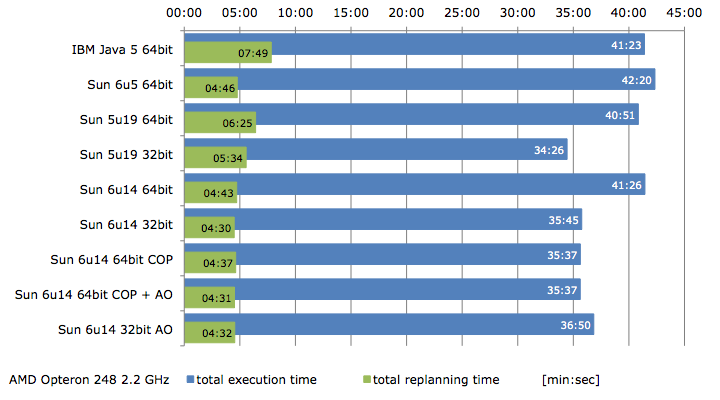
\includegraphics[width=0.75\linewidth]{figures/benchmarks/benchmark1}
\caption{The average of two runs of the benchmark for each configuration.}
\label{fig:Benchmark01}
\end{figure}
What can be observed is the huge difference of execution time in general between 32-bit and 64-bit versions of the virtual machines. The \emph{compressed object pointers} (COP) feature of Suns JVM 6u14 seems to compensate for this nicely, making the 64-bit version about the same speed than the 32-bit version. The aggressive optimization options (AO) on the other hand doesn't seem to influence the performance of MATSim drastically.

While the difference between Suns Java 5 and Java 6 versions in the total execution time seem more or less random, there seems to be a performance improvement for the multithreaded replanning part by changing from Java 5 to Java 6. Interestingly, despite IBM's worse multithreaded performance, it is able to catch up in the single-threaded parts to come in with a similar total execution time than Sun's 64-bit JVMs.

The benchmark was also run on other server machines:

\begin{itemize}
\item Servers with two Dual-Core AMD Opteron 2222 processors, running at 3.0 GHz; date of purchase winter 2007/2008 (very similar architecture than the previously tested AMD Opteron 248 systems, just \emph{newer} with higher clocked CPU).
\item Servers with Intel Xeon X5355 Quad-Core processors, clocked at 2.66 GHz, 8 MB L2 cache, built with 65 nm technology.
\item Servers with Intel Xeon E5430 Quad-Core processors, clocked at 2.66 GHz, 12 MB L2 cache, built with 45 nm technology.
\item Servers with Intel Xeon E5530 Quad-Core processors, clocked at 2.4 GHz, 8 MB L3 cache, 45 nm technology, Nehalem architecture.
\item Servers with Intel Xeon E7540 Hex-Core processors, clocked at 2.0 GHz, 18 MB L3 cache, 45 nm technology, Nehalem architecture, DDR3 RAM.
\end{itemize}
Comparing (in Figure~\ref{fig:Benchmark02}) the AMD servers running at 2.2 GHz and 3.0 GHz, the most obvious difference is the time for the replanning, explainable by the different number of cores the machines have. 
\begin{figure}[h]
\centering
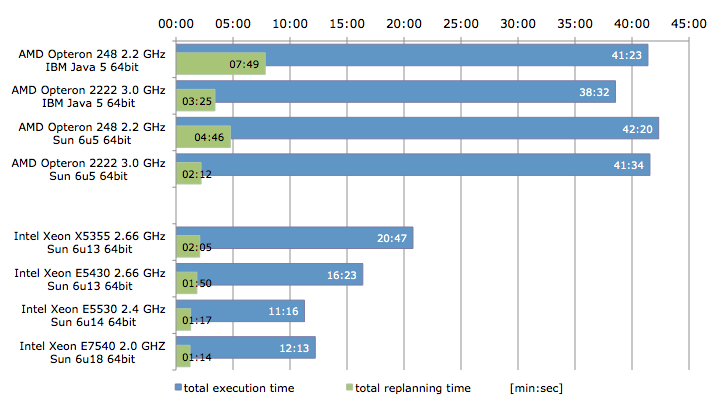
\includegraphics[width=0.75\linewidth]{figures/benchmarks/benchmark2}
\caption{The average of two runs of the benchmark for different servers.}
\label{fig:Benchmark02}
\end{figure}
Interestingly, the remaining execution time didn't really improve by the change in CPU speed, leading to the guess that the performance of the memory controller or the memory bus is limiting the speed of MATSim (both AMD servers seem to have a front side bus of 1000 MHz).

The Intel servers were massively faster than the AMD machines. We do not yet know if it's the different memory controller, faster memory bus, or if Sun's JDK is just more optimized for Intel processors. Anyway, the difference is striking. And each newer generation of Intel processors seems to deliver a real performance upgrade, even when running at a lower clock-speed.

At last, the benchmark was also run on some of our laptop machines: An Apple MacBook Pro with a Intel Core 2 Duo processor clocked at 2.33 GHz (model from fall 2006), running Mac OS X 10.5.7, and an IBM/Lenovo Laptop with the same Intel Core 2 Duo processor, 2.33 GHz, running a Gentoo 64-bit Linux (Kernel 2.6.28). Both laptops have a front side bus of 667 MHz, so from a technical view point they are very similar.

On the Apple MacBook Pro, the following Java Virtual Machines were used:

\begin{description}
\item[Apple JVM 5u16 32bit]\quad The default Java 5 version on Mac OS provided by Apple.
\item[Apple JVM 6u7 64bit]\quad The default Java 6 version on Mac OS provided by Apple.
\item[Soylatte 6u3 32bit]\quad An early port of OpenJDK 6, identifying itself as \texttt{1.6.0\_03-p3; Sun Microsystems Inc.; mixed mode; 32-bit}, provided by \href{http://landonf.bikemonkey.org/static/soylatte/}{Landon Fuller}.
\end{description}
On the Lenovo Laptop, an OpenJDK 6u0 64-bit JVM was used.
\begin{figure}[h]
\centering
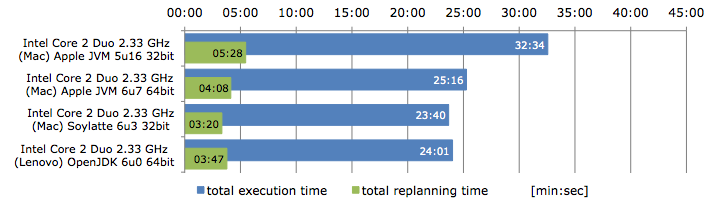
\includegraphics[width=0.75\linewidth]{figures/benchmarks/benchmark3}
\caption{The average of two runs of the benchmark for laptops.}
\label{fig:Benchmark03}
\end{figure}
Surprisingly, Apple pulled the trick to make their 64-bit Java 6 a lot faster than the older 32-bit Java 5—well, it could also mean that their Java 5 offering was just very slow\ldots The Mac-port of OpenJDK 6 (\emph{Soylatte}) is even a bit faster, but that may be likely due to the difference between 64-bit and 32-bit.

Are you able to run the MATSim benchmark even faster? Please tell us so! We're very interested in your benchmark results.

\subsubsection{Memory usage comparison}
MATSim writes out information about memory usage from time to time into the logfile. Plotting this information gives a jagged line running from left to right. Heights and lows in the plot can be explained with the Java Garbage Collector, only freeing up the memory from time to time. Still, one can guess the absolute minimum of memory required by MATSim by looking at the lower parts of the curve (that's then when a Garbage Collection just ran, showing all the memory that could not be collected).

Comparing the memory consumption in Sun's (currently) latest Java VM version holds no real surprises.
\begin{figure}[h]
\centering
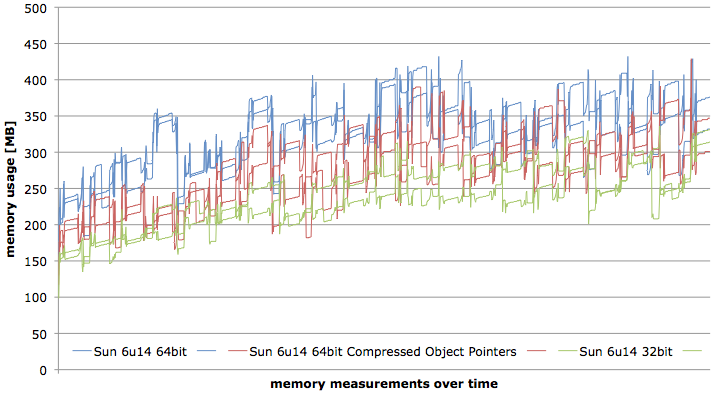
\includegraphics[width=0.75\linewidth]{figures/benchmarks/benchmark_memory}
\caption{Memory usage over iterations.}
\label{fig:Benchmark04}
\end{figure}

It can be clearly seen that the 64-bit JVM uses the largest amount of memory, due to the fact that each object pointer takes up 8 bytes. The 32-bit JVM uses the least memory. The 64-bit JVM with compressed object pointers seems to lie somewhere in between—although I would have expected it to be comparable to the 32-bit JVM, it seems that it still uses a bit more memory for unknown reasons. Anyway, it comes in handy to know that one can load now larger scenarios on a 32GB (or less) machine. The memory savings, compared to a 64-bit JVM without compressed object pointers, should be even bigger the larger the scenario is or the more details the simulated network has, so this feature really looks promising.
 
So, by how much can you improve your MATSim simulation's performance?

\section{Speeding up your own MATSim runs}
There are a few things you can try to speed up your simulation runs. The following hints are not in any specific order.%% {\color{red}(are they?)}.

\subsection{Use an up-to-date Java version}
Java 7 usually performs better than Java 6.

\subsection{Use compressed object pointers in 64-bit JVM}

Since Sun Java 6, Update 14, if you use a 64-bit JVM and use at most 32 GB of RAM, start Sun's Java virtual machine with the argument 
\begin{lstlisting}{language=xml}
-XX:+UseCompressedOops
\end{lstlisting}
This reduces the size of object pointers to 32 bit, making many pointer operations a lot faster than when they were 64 bit long, while still supporting heap sizes larger than 2 GB (what a regular 32-bit JVM would do). See the \href{http://www.oracle.com/technetwork/java/javase/6u14-137039.html}{Java SE 6 Update 14 Release Notes} for more details. In addition, we observed notable speed-ups in the region of 10\% in the run time of MATSim. Since Java SE 6 Update 23 and in Java 7, this option is enabled by default.

\subsection{Parallelization}
When running a MATSim simulation, unused cores can be utilized to make the simulation faster. There are now three ways to improve performance using parallelization, and each can be switched on or off separately.

\subsubsection{Event handling}\label{sec:ParallelEventsHandling}
The event handler which is used by default, is running in the same thread as the simulation. For this reason, you can switch on parallel event handling by adding the \texttt{parallelEventHandling} module to the MATSim \texttt{Config} XML file as follows:
\begin{lstlisting}{language=xml}
<module name="parallelEventHandling">
    <param name="numberOfThreads" value="1" />
</module>
\end{lstlisting}
The only required parameter in this module is \texttt{numberOfThreads}. The value of this parameter specifies how many threads (cores) should be assigned to handling events.

There is an additional optional parameter \texttt{estimatedNumberOfEvents}, which can be optimized to your simulation resulting in slightly faster runs. But its usage requires an estimate of the number of events which will occur in one iteration.
\begin{lstlisting}{language=xml}
<param name="estimatedNumberOfEvents" value="5000000" />
\end{lstlisting}
The following are some hints to consider and pitfalls to avoid:
\begin{itemize}
\item Don't make any  assumptions on the order, in which the handlers are executed (as they are executed in parallel).
\item Don't write the data in one handler and read that data in a different handler. Although this is possible, special care is required as synchronization between threads is needed for this. Furthermore this could lead to a degradation of the speed up.
\item There is no point in using parallel event handling, if you have just one core available on your machine.
\item Always make sure, that one thread is needed for the single cpu simulation. This means, if you have 4 cores, you can set the parameter 'numberOfThreads' to maximum 3.
\item If 2 handlers have been added to the simulation, then there is no point in assigning 3 threads to parameter \texttt{numberOfThreads}, because it won't make the simulation faster (but rather could slow it down in some cases).
\item The number of handlers can be bigger than \texttt{numberOfThreads}. In this case automatically if possible, each thread is assigned the same number of handlers. 
\item If the simulation is quite slow (compared to event handling), you won't be able to make full use of parallel event handling.
\end{itemize} 
The actual speed up you get depends on many factors, especially on those in the aforementioned hints and pitfalls. Experiments on a 16 core machine with different numbers of handlers have shown that the parallel event handler can reduce the simulation time with a very low overhead. Some Java specific implementation aspects of \emph{JDEQSim} and the \texttt{parallelEventHandling} module are described in the paper by Waraich, R., D. Charypar, M. Balmer and K.W. Axhausen (2009) Performance improvements for large scale traffic simulation in MATSim, paper presented at the 9th Swiss Transport Research Conference, Ascona, September 2009. This paper can be downloaded \href{http://www.ivt.ethz.ch/vpl/publications/reports/ab565.pdf}{here}. 

\subsubsection{Mobility simulation}\label{sec:ParallelQsim}
\authorsOfCode{C. Dobler, IVT}
\maintainers{C. Dobler, IVT}

There is a parallel version of the qsim. Analysis of performance and structure of (non parallel) qsim shows:
\begin{itemize}
\item Simulation of movement on links and over nodes is most time consuming.
\item Within a timestep actions on nodes and links can be simulated on parallel threads with low additional synchronization effort.
\end{itemize}

The parallel qsim is based on the existing qsim and can be used by just adding a new parameter to a scenario configuration file (see ). First performance measurements show promising results, and a working paper will be published in Q2 2010. A structural description of the parallel qsim is shown in Figure~\ref{fig:ParallelQsim}.
\begin{figure}[htp]
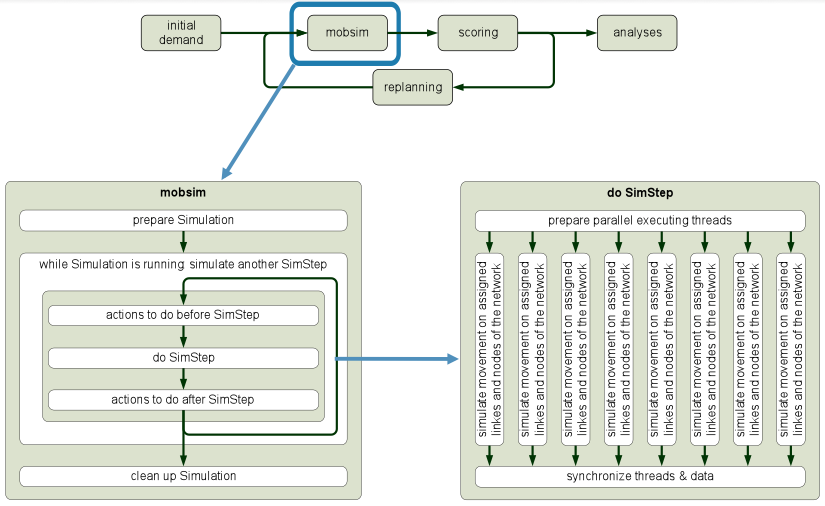
\includegraphics[width=\textwidth]{figures/qsimParallel/parallelqsim.png}
\caption{Design of the parallel qsim.}\label{fig:ParallelQsim}
\end{figure}

To activate it, ensure that a \texttt{qsim} module is added to the config XML file of MATSim, and set the \texttt{numberOfThreads} parameter as follows:
\begin{lstlisting}{language=xml}
<module name="qsim">
   ...
   <param name="numberOfThreads" value="5"/>
</module>
\end{lstlisting}
or however many number of threads you want to use. An unlimited number of threads will \emph{not} make your simulation run infinitely fast. A performance \emph{decrease} can actually occur, depending on the scenario size. Refer to Christoph Dobler's thesis (Chapter 5) for a complete discussing in this regard. Figure~\ref{fig:QsimPerformance} shows an estimation of the (optimal) number of threads required for a given scenario size (expressed as number of events generated).
\begin{figure}[h]
\centering
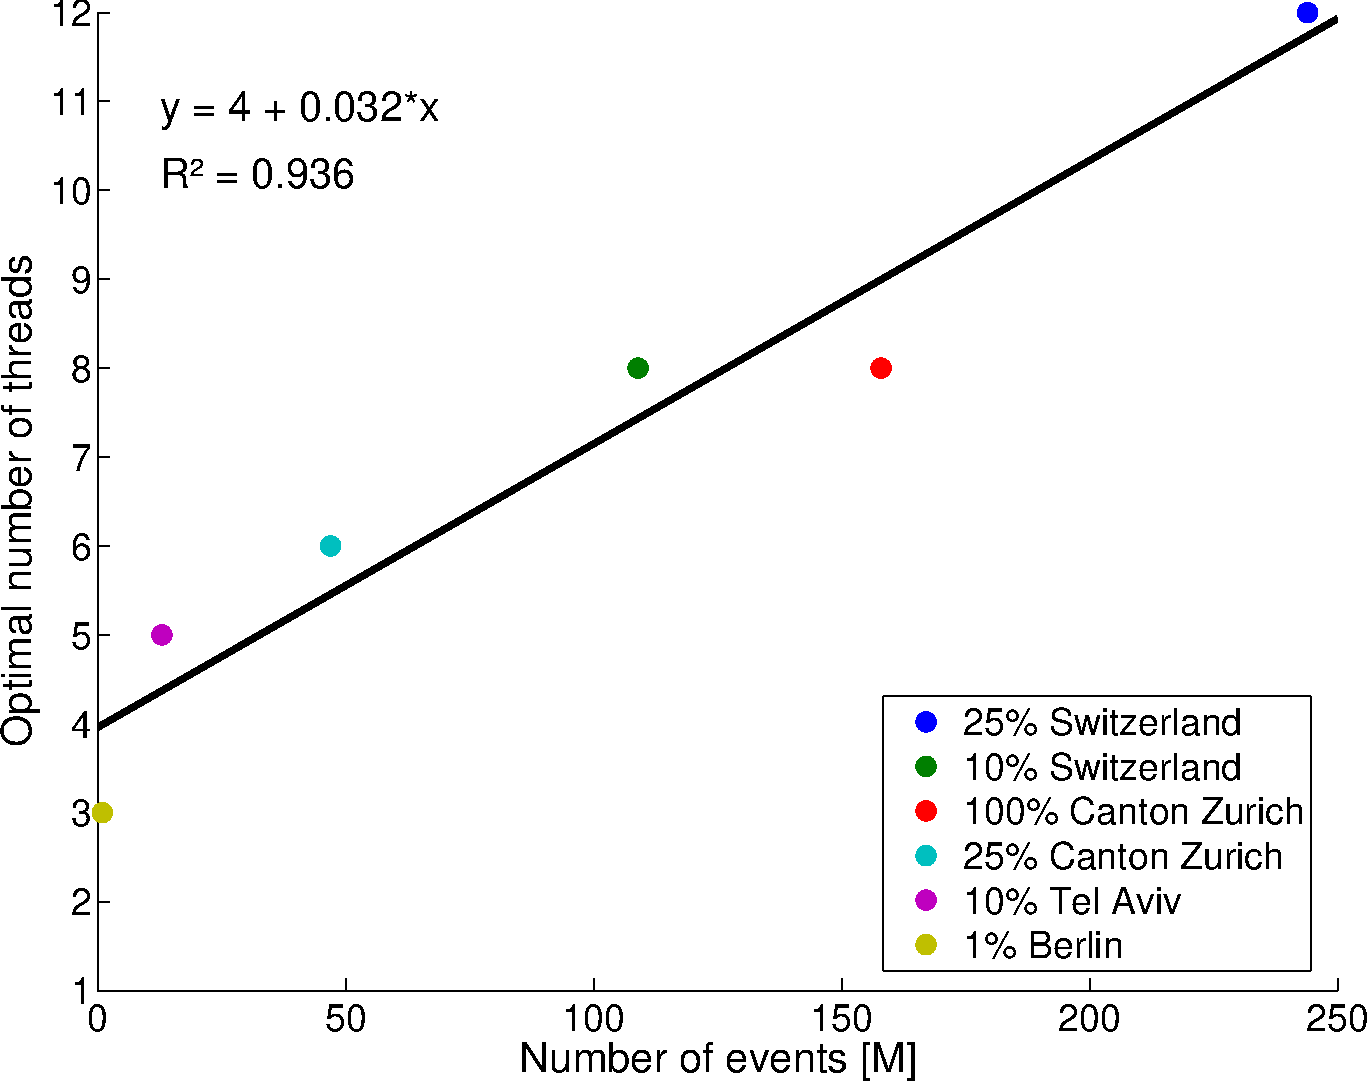
\includegraphics[width=0.6\linewidth]{figures/benchmarks/EventsVsSpeedUp}
\caption{Estimated number of threads to use for a given scenario size.} 
\label{fig:QsimPerformance}
\label{figureLabel}
\end{figure}

Dobler, C. (2013). Travel behaviour modelling for scenarios with exceptional events --- methods and implementations, Dissertation, IVT, ETH Zurich, Zurich. Available online \href{http://e-collection.library.ethz.ch/view/eth:7633}{here}.

\subsubsection{Replanning}
To set the simulation to parallelize the replanning phase, the following parameter must be set the the \texttt{global} module of the config XML file:
\begin{lstlisting}{language=xml}
<module name="global">
  ...
  <param name="numberOfThreads" value="8" />
</module>
\end{lstlisting}

\subsection{Limit the writing of events}
Writing the simulation events to files in each iteration not only consumes a lot of disk space, but also a considerable amount of time. Add the following parameter to your configuration to restrict writing events to certain iterations:
\begin{lstlisting}{language=xml}
<module name="controler">
  ...
  <param name="writeEventsInterval" value="10" />
</module>
\end{lstlisting}

\subsection{Use faster routing algorithms}
By default, MATSim uses a routing algorithm based on Dijkstra's shortest path algorithm. But MATSim also includes a faster routing algorithm, based on the A$^{\star}$ algorithm with landmarks. To use this routing algorithm, add the following configuration parameter to your configuration file:
\begin{lstlisting}{language=xml}
<module name="controler">
  ...
  <param name="routingAlgorithmType" value="AStarLandmarks" />
</module>
\end{lstlisting}

\subsection{Comparing parallelisation options}
The following shows two different benchmarks using jdeqsim (Section~\ref{sec:Jdeqsim}), parallel events handling (Section~\ref{sec:ParallelEventsHandling}), or both. The first benchmark, Figure~\ref{fig:JdeqsimTime}, uses the ivtch-osm network (approximately 60,000 links), while the second one, Figure~\ref{fig:JdeqsimTime-navteq}, uses a navteq network with much more links.

\subsubsection{QueueSim versus JDEQSim using parallel events handling}
Zrh 10\%, ivtch-osm network; computing times per iteration (computer = cluster4 = 2x ``Dual-Core AMD Opteron Processor 2222'', 3.0 GHz, 1000 MHz FSB).  Runs 669, 676, 678, 679
\begin{figure}[h]
\centering
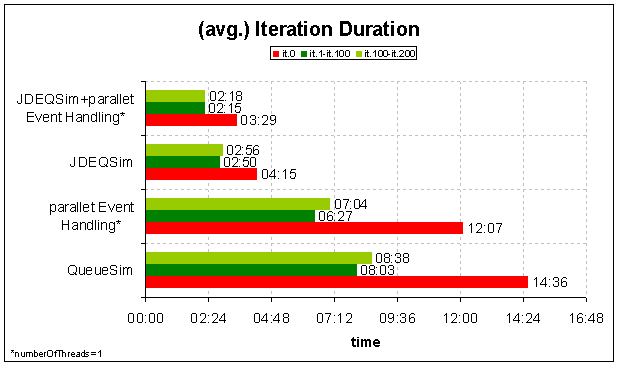
\includegraphics[width=0.75\linewidth]{figures/benchmarks/jdeqsimtime}
\caption{Using the ivtch-osm network.}
\label{fig:JdeqsimTime}
\end{figure}

Computing times per Iterations.  Scenario = navteq network of Switzerland; computer = cluster4 = servers with 2x ``Dual-Core AMD Opteron Processor 2222'', 3.0 GHz, 1000 MHz FSB.
\begin{figure}[h]
\centering
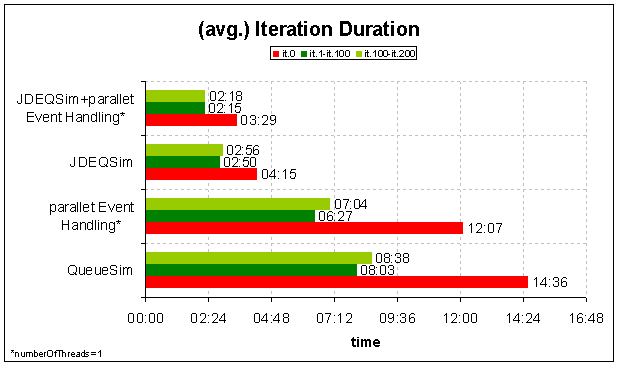
\includegraphics[width=0.75\linewidth]{figures/benchmarks/jdeqsimtime}
\caption{Using the ivtch-osm network.}
\label{fig:JdeqsimTime-navteq}
\end{figure}


\NextFile{PolicyMeasures.html}
\chapter{Specific applications}

\authorsOfDoc{Kai Nagel}

A discussion of policy measures that can be investigated with matsim is under \href{http://matsim.org/policy-measures}{matsim.org/policy-measures}  . It is not in the user section but in the developer section of  the documentation since, at this point, many of those measures need additional coding. 

Clearly, something like adding or removing lanes or  links can be investigated without any coding.  Examples for use cases and policy measures that can be investigated without coding can be found in the following.

\section{MATSim as tool for dynamic traffic assigment (DTA)}

%%A MATSim iteration can be seen as consisting of the following steps:
%%\begin{itemize}
%%\item Physical simulation ($=$ network loading) and scoring
%%\item Innovation and plans removal ($=$ modification of the choice sets)
%%\item Choice
%%\end{itemize}

A typical MATSim use case is the use as dynamic traffic assignment (DTA) tool.  In DTA, trips are given by departure time, departure location, and destination, and the task of DTA is to find routes.  The task is typically solved by iterating between network loading and routing; possible outcomes are a Nash equilibrium (no traveller can improve its score/utility by switching to a different route) or SUE (so-called stochastic user equilibrium).

In order to use MATSim for this, one needs to convert each trip into a pseudo-person.  I call this ``pseudo''-person since it does not correspond to a real person; rather, it is probably that multiple trips belong to one person.  The input file would look something like
\begin{lstlisting}{language=xml}
<population>
<person>
   <plan>
      <act type="dummy" x="<dp loc x>" y="<dp loc y>" endTime="<dp time>" />
      <act type="dummy" x="<dest x>" y="<dest y>" />
   </plan>
</person>
<person>
...
</population>
\end{lstlisting}
where

\begin{tabularx}{\hsize}{rX}
\verb$dummy$ & arbitrary activity type, see below \\
\verb$<dp time>$ & starting time of trip \\
\verb$<dp loc x>$ & x coordinate of departure location \\
\verb$<dest x>$ & x coordinate of destination \\
\end{tabularx}

Alternatively, one can use link ids for departure locations and destinations:
\begin{lstlisting}{language=xml}
<population>
<person>
   <plan>
      <act type="dummy" link="<link id>" endTime="<dp time>" />
      <act type="dummy" link="<link id>" x="<dest x>" y="<dest y>" />
   </plan>
</person>
<person>
...
</population>
\end{lstlisting}

Note that MATSim trips start on links, not at nodes.  You somehow have to convert this.

This file, together with the appropriate network file and an appropriate config file, will serve as input to MATSim.  The config file will look something like
\begin{lstlisting}{language=xml}
<module name="network" >
	<param name="inputNetworkFile" value="..." /> 
</module>
<module name="plans" >
	<param name="inputPlansFile" value="..." />
</module>
<module name="controler" >
	<param name="firstIteration" value="0" />
	<param name="lastIteration" value="100" />
</module>
<module name="planCalcScore" >
	<param name="activityType_0" value="dummy" />
        <!-- (same activity type as used in plans file) -->
</module>
<module name="strategy" >
	<param name="Module_1" value="ChangeExpBeta" />
	<param name="ModuleProbability_1" value="0.9" />

	<param name="Module_2" value="ReRoute" />
	<param name="ModuleProbability_2" value="0.1" />
</module>
\end{lstlisting}

The overall calling syntax is something like
\begin{lstlisting}
java -cp matsim.jar -Xmx2000m org.matsim.run.Controler config.xml 
\end{lstlisting}

There is a corresponding example in recent releases; it should run (in the release directory) with 
\begin{lstlisting}
java -cp matsim-0.5.0.jar org.matsim.run.Controler examples/tutorial/config/example5-config.xml
\end{lstlisting}
\verb$-Xmx2000m$ needs to be added when the scenario gets larger.

%%%%%%%%%%%%%%%%%%%%%%%%%%%%%%%%%%%%%%%%%%%%
%%%%%%%%%%%%%%%%%%%%%%%%%%%%%%%%%%%%%%%%%%%%
\section{Including one's own upstream module}
\label{sec:including-ones-own}

There is the possibility to call one's own upstream plans modification module.  The config is something like
\begin{lstlisting}{language=xml}
<module name="strategy" >
	<param name="Module_1" value="ChangeExpBeta" />
	<param name="ModuleProbability_1" value="0.9" />

	<param name="Module_2" value="ReRoute" />
	<param name="ModuleProbability_2" value="0.1" />

	<param name="ModuleProbability_3" value="0.1" />
	<param name="ModuleExePath_3" value="<some executable>" />
</module>
\end{lstlisting}
where

\begin{tabularx}{\hsize}{rX}
\verb$<some executable>$ & is the (unix) call of some external executable, e.g.\ a shell script \\
\end{tabularx}

The external executable will be called with a config file as an argument.  The config file will contain, e.g., the iteration number, the full path name to the input plans file, the full path name to the output plans file, and the full path name to the (txt) events file.\footnote{%
%
If you would prefer the xml events here, please let us know, this is easy to change, in particular when someone else tries it out.
%
}
The input plans file are the plans that come from MATSim.  The output plans is the place where the modified plans file should be written to  The events are the information on which the external module can base its computations.

%%%%%%%%%%%%%%%%%%%%%%%%%%%%%%%%%%%%%%%%%%%%
%%%%%%%%%%%%%%%%%%%%%%%%%%%%%%%%%%%%%%%%%%%%
\section{MATSim for network loading only}

Maybe one wants to use MATSim only for the network loading.  In this case, the plans file needs to look something like
\begin{lstlisting}{language=xml}
<population>
<person>
   <plan>
      <act type="dummy" x="<dp loc x>" y="<dp loc y>" endTime="<dp time>" />
      <leg mode="car">
         <route> 18 24 45 </route>
      </leg>
      <act type="dummy" x="<dest x>" y="<dest y>" />
   </plan>
</person>
<person>
...
</population>
\end{lstlisting}
where the route section needs to contain the route information. \kai{chk plans v5 fmt}

The config file will be something like
\begin{lstlisting}{language=xml}
<module name="network" >
	<param name="inputNetworkFile" value="..." /> 
</module>
<module name="plans" >
	<param name="inputPlansFile" value="..." />
</module>
<module name="controler" >
	<param name="firstIteration" value="0" />
	<param name="lastIteration" value="0" />
</module>

<!-- don't know if the following is necessary: -->
<module name="planCalcScore" >
	<param name="activityType_0" value="dummy" />
        <!-- (same activity type as used in plans file) -->
</module>
\end{lstlisting}

The overall calling syntax is again something like (*)
\begin{lstlisting}
java -cp matsim.jar -Xmx2000m org.matsim.run.controler config.xml 
\end{lstlisting}

There are two obvious options how this can be used:
\begin{itemize}
\item There is some external mechanics, e.g.\ some external script, which keeps calling MATSim from the command line as in (*), and then takes the output events in order to update plans.
\item One uses the MATSim iteration mechanics, as described in Sec.~\ref{sec:including-ones-own}, to call an external module, which also modifies routes. 
\end{itemize}





% Local Variables:
% mode: latex
% mode: reftex
% mode: visual-line
% TeX-master: "../user-guide.tex"
% comment-padding: 1
% fill-column: 9999
% End: 

% no longer include extensions into user guide, decided at devmtg2013. mr/oct13
%\include{chapters/extensions}

%\appendix
%\chapter*{Appendices}
%\addcontentsline{toc}{chapter}{Appendices}
%\markboth{Appendices}{}%fix headers



%%%%%%%%%%%%%%%%%%%%%%%%%%%%%%%%%%%%%%%%%%%%
%%%%%%%%%%%%%%%%%%%%%%%%%%%%%%%%%%%%%%%%%%%%


\umbruch
%%%%%%%%%%%%%%%%%%%%%%%%%%%%%%%%%%%%%%%%%%%%
%%%%%%%%%%%%%%%%%%%%%%%%%%%%%%%%%%%%%%%%%%%%
%%%%%%%%%%%%%%%%%%%%%%%%%%%%%%%%%%%%%%%%%%%%
%%%%%%%%%%%%%%%%%%%%%%%%%%%%%%%%%%%%%%%%%%%%
\end{document}



% Local Variables:
% mode: latex
% mode: reftex
% mode: visual-line
% comment-padding: 1
% fill-column: 999
% End: 
